%Este trabalho está licenciado sob a Licença Atribuição-CompartilhaIgual 4.0 Internacional Creative Commons. Para visualizar uma cópia desta licença, visite http://creativecommons.org/licenses/by-sa/4.0/deed.pt_BR ou mande uma carta para Creative Commons, PO Box 1866, Mountain View, CA 94042, USA.

\chapter{Derivadas}\label{cap_deriv}
\thispagestyle{fancy}

\section{Derivada no ponto}\label{cap_deriv_sec_derivpt}

Nesta seção, vamos estudar a noção de {\bf derivada de uma função em um ponto}. Começamos pelas noções de {\bf reta secante} e de {\bf reta tangente} ao gráfico de uma função. Em seguida, estudamos as noções de {\bf taxa de variação média} e {\bf taxa de variação instantânea}. Por fim, definimos a derivada de uma função em um ponto.

\subsection{Reta secante e reta tangente}

\begin{flushright}
  [YouTube] | [Vídeo] | [Áudio] | \href{https://phkonzen.github.io/notas/contato.html}{[Contatar]}
\end{flushright}

Definimos a {\bf reta secante} ao gráfico de uma dada função $f$ pelos pontos $x_0$ e $x_1$, $x_0\neq x_1$, como sendo a reta determinada pela equação
\begin{equation}
  {\color{blue}y = \frac{f(x_1)-f(x_0)}{x_1-x_0}(x-x_0)+f(x_0)}.
\end{equation}
Isto é, é a reta que passa pelos pontos $(x_0,f(x_0))$ e $(x_1,f(x_1))$. Veja a Figura \ref{fig:retsectg}. Observemos que o coeficiente angular da reta secante é
\begin{equation}
  {\color{blue}m_{\text{sec}} = \frac{f(x_1)-f(x_0)}{x_1-x_0}}.
\end{equation}

\begin{figure}[H]
  \centering
  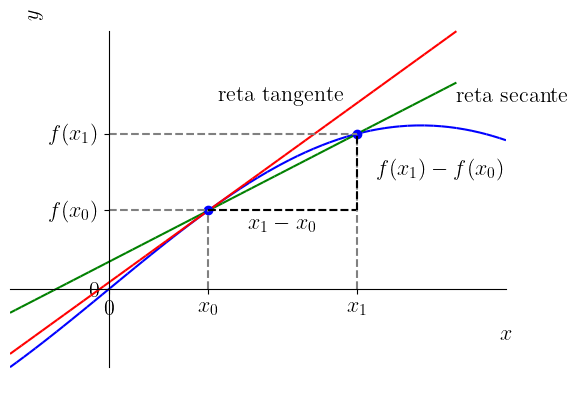
\includegraphics[width=0.8\textwidth]{./cap_deriv/dados/fig_retsectg/fig}
  \caption{Esboços de uma reta secante (verde) e da reta tangente (vermelho) ao gráfico de uma função.}
  \label{fig:retsectg}
\end{figure}

A {\bf reta tangente} ao gráfico de uma função $f$ em $x=x_0$ é a reta que passa pelo ponto $(x_0, f(x_0))$ e tem coeficiente angular
\begin{equation}\label{eq:mtg}
  {\color{blue}m_{\text{tg}} = \lim_{x_1\to x_0} \frac{f(x_1)-f(x_0)}{x_1-x_0}}.
\end{equation}
Isto é, a reta de equação
\begin{equation}
  {\color{blue}y = m_{\text{tg}}(x-x_0)+f(x_0)}.
\end{equation}
Menos formal, é a reta limite das retas secantes ao gráfico da função pelos pontos $x_0$ e $x_1$, quando $x_1\to x_0$. Veja a Figura \ref{fig:retsectg}.

\begin{obs}
  Fazendo a mudança de variável $h = x_1-x_0$, temos que \eqref{eq:mtg} é equivalente a
  \begin{equation}
    {\color{blue}m_{\text{tg}} = \lim_{h\to 0} \frac{f(x_0+h)-f(x_0)}{h}}.
  \end{equation}
  De fato, da mudança de variável, temos que $x_1 = x_0+h$ e quando $x_1\to x_0$, temos que $h = x_1-x_0\to 0$. Ou seja,
  \begin{align}
    m_{\text{tg}} &= \lim_{x_1\to x_0} \frac{f(x_1)-f(x_0)}{x_1-x_0}\\
                  &= \lim_{h\to 0} \frac{f(x_0+h)-f(x_0)}{h}.
  \end{align}
\end{obs}

\begin{ex}
  Seja $f(x)=x^2$ e $x_0 = 1$. O coeficiente angular da reta secante ao gráfico de $f$ pelos pontos $x_0=1$ e $x_1 = 2$ é
  \begin{align}
    m_{\text{sec}} &= \frac{f(x_1)-f(x_0)}{x_1-x_0}\\
                   &= \frac{f(2) - f(1)}{2-1}\\
                   &= \frac{4-1}{1} = 3.
  \end{align}
  Logo, a reta secante ao gráfico de $f$ pelos pontos $x_0=1$ e $x_1=2$ tem equação
  \begin{gather}
    y = m_{\text{sec}}(x-x_0) + f(x_0) \\
    y = 3(x-1)+f(1) \\
    y = 3x - 2.
  \end{gather}
  Na Figura \ref{fig:cap_deriv_ex_rt_x2}, temos os esboços dos gráfico da função e da reta secante (verde).
  
  \begin{figure}[H]
    \centering
    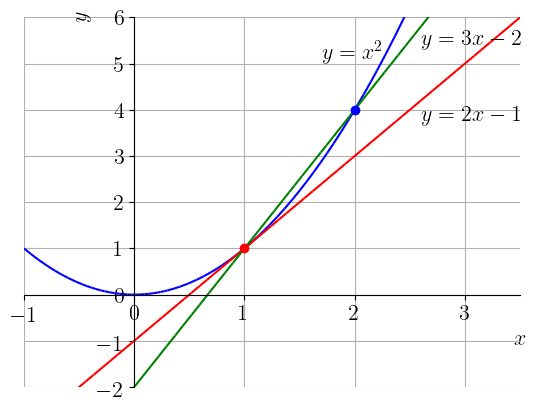
\includegraphics[width=0.7\textwidth]{./cap_deriv/dados/fig_cap_deriv_ex_rt_x2/fig}
    \caption{Esboços dos gráficos de $f(x)=x^2$ (azul), da reta secante pelos pontos $x_0=1$ e $x_1=2$ (verde) e da reta tangente ao gráfico de $f$ no ponto $x_0 = 1$ (vermelho).}
    \label{fig:cap_deriv_ex_rt_x2}
  \end{figure}

  Agora, o coeficiente angular da reta tangente ao gráfico de $f$ no ponto $x_0$ é
  \begin{align}
    m_{\text{tg}} &= \lim_{h\to 0} \frac{f(x_0+h)-f(x_0)}{h}\\
                  &= \lim_{h\to 0} \frac{(1+h)^2-1}{h}\\
                  &= \lim_{h\to 0} \frac{1+2h+h^2-1}{h}\\
                  &= \lim_{h\to 0} \frac{2+h}{1} = 2.
  \end{align}
  Assim sendo, a reta tangente ao gráfico de $f(x)=x^2$ no ponto $x_0=1$ tem coeficiente angular $m_{\text{tg}} = 2$ e equação
  \begin{equation}
    y = 2(x-1)+1 = 2x-1.
  \end{equation}
  Na Figura \ref{fig:cap_deriv_ex_rt_x2}, temos os esboços dos gráfico da função e da reta tangente (vermelho).
  
  \ifispython
  Com o {\python}+{\sympy}, podemos obter a expressão da reta secante com os seguintes comandos:
  \begin{lstlisting}
    In : from sympy import *
    ...: x,y = symbols('x,y')
    ...: x0 =  1
    ...: x1 = 2
    ...: f = lambda x: x**2
    ...: msec = (f(x1)-f(x0))/(x1-x0)
    ...: Eq(y, msec*(x-x0)+f(x0))
    Out: Eq(y, 3.0*x - 2.0)
  \end{lstlisting}
  A expressão da reta tangente pode ser obtida com os seguintes comandos:
  \begin{lstlisting}
    In : from sympy import *
    ...: x,y = symbols('x,y')
    ...: h = Symbol('h')
    ...: x0 = 1
    ...: f = lambda x: x**2
    ...: mtg = limit((f(x0+h)-f(x0))/h, h, 0)
    ...: Eq(y, mtg*(x-x0)+f(x0))
    ...: 
    Out: Eq(y, 2*x - 1)
  \end{lstlisting}
  \fi
\end{ex}

\subsection{Taxa de variação}

\begin{flushright}
  [YouTube] | [Vídeo] | [Áudio] | \href{https://phkonzen.github.io/notas/contato.html}{[Contatar]}
\end{flushright}

A {\bf taxa de variação média} de uma função $f$ quando $x$ varia de $x_0$ a $x_1$ é definida como
\begin{equation}
  \frac{\Delta y}{\Delta x} := \frac{f(x_1)-f(x_0)}{x_1-x_0}. 
\end{equation}
Desta deriva-se a {\bf taxa de variação instantânea} de $f$ no ponto $x_0$, a qual é definida como
\begin{align}
  \left.\frac{\dd f}{\dd x}\right|_{x=x_0} &:= \lim_{x\to x_0} \frac{f(x)-f(x_0)}{x-x_0}\\
                             &= \lim_{h\to 0} \frac{f(x_0+h)-f(x_0)}{h}.
\end{align}
Em muitas áreas do conhecimento, estas taxa recebem nomes específicos.

\begin{ex}
  Seja $s = s(t)$ a função distância percorrida por um objeto no tempo. A {\bf velocidade média} (taxa de variação média da distância) do tempo $t_0$ ao tempo $t_1$ é
  \begin{equation}
    \frac{\Delta s}{\Delta t} = \frac{s(t_1)-s(t_0)}{t_1-t_0}.
  \end{equation}
  Por exemplo, se $s(t) = 15t^2+t$ (km), então a velocidade média do objeto entre $t_0=1$h e $t_1=3$h é
  \begin{align}
    \frac{\Delta s}{\Delta t} &= \frac{(15t_1^2+t_1)-(15t_0^2+t_0)}{t_1-t_0}\\
                              &= \frac{15\cdot 3^2+3-(15\cdot 1^2+1)}{3-1}\\
                              &= \frac{135+3-15-1}{2}\\
                              &= 61~\frac{\text{km}}{\text{h}}.
  \end{align}

  A {\bf velocidade} (taxa de variação instantânea da distância) no tempo $t_0=1$ é
  \begin{align}
    \left.\frac{\dd s}{\dd t}\right|_{t=t_0} &= \lim_{h\to 0} \frac{s(t_0+h)-s(t_0)}{h} \\
                                             &= \lim_{h\to 0} \frac{15(t_0+h)^2+(t_0+h)-\left(15t_0^2+t_0\right)}{h}\\
                                             &= \lim_{h\to 0} \frac{15t_0^2+30t_0h+15h^2+t_0+h-15t_0^2-t_0}{h}\\
                                             &= \lim_{h\to 0} \frac{30t_0h+15h^2+h}{h}\\
                                             &= \lim_{h\to 0} 30t_0 + 15h + 1 \\
                                             &= 30t_0+1 = 31~\frac{\text{km}}{\text{h}}.
  \end{align}
\end{ex}

\begin{ex}
  Seja $c(x) = \sqrt{x}$ (milhões de reais) o custo da produção em uma empresa em função do número de unidades produzidas (milhares). O {\bf custo médio da produção} de $x_0=4$ a $x_1=9$ é
  \begin{align}
    \frac{\Delta c}{\Delta x} &= \frac{c(x_1)-c(x_0)}{x_1-x_0}\\
                              &= \frac{\sqrt{x_1}-\sqrt{x_0}}{x_1-x_0}\\
                              &= \frac{\sqrt{9}-\sqrt{4}}{9-4}\\
                              &= \frac{3-2}{5} \\
                              &= 0,2~\frac{\text{R\$}}{\text{un}}.
  \end{align}

  O {\bf custo marginal} (taxa de variação instantânea do custo) quando a empresa está produzindo $x_0=4$ milhões de unidades é
  \begin{align}
    \left.\frac{\dd c}{\dd x}\right|_{x=x_0=4} &= \lim_{h\to 0} \frac{\sqrt{x_0+h}-\sqrt{x_0}}{h}\\
                                               &= \lim_{h\to 0} \frac{\sqrt{x_0+h}-\sqrt{x_0}}{h}\cdot \frac{\sqrt{x_0+h}+\sqrt{x_0}}{\sqrt{x_0+h}+\sqrt{x_0}}\\
                                               &= \lim_{h\to 0} \frac{x_0+h-x_0}{h(\sqrt{x_0+h}+\sqrt{x_0})}\\
                                               &= \lim_{h\to 0} \frac{1}{\sqrt{x_0+\cancelto{0}{h}}+\sqrt{x_0}}\\
                                               &= \frac{1}{2\sqrt{x_0}} = \frac{\sqrt{x_0}}{2x_0}\\
                                               &= \frac{\sqrt{4}}{2\cdot 4} = 0,25~\frac{\text{R\$}}{\text{un}}.
  \end{align}
\end{ex}

\begin{obs}
  Analogamente a custo marginal, temos as noções de rendimento marginal e lucro marginal.
\end{obs}

\subsection{Derivada em um ponto}

\begin{flushright}
  [Vídeo] | [Áudio] | \href{https://phkonzen.github.io/notas/contato.html}{[Contatar]}
\end{flushright}

A {\bf derivada} de uma função $f$ {\bf em um ponto} $x=x_0$ é denotada por $f'(x_0)$ ou $\displaystyle \frac{\dd f}{\dd x}(x_0)$ e é definida por
\begin{equation}
  f'(x_0) = \left.\frac{\dd f}{\dd x}\right|_{x=x_0} := \lim_{h\to 0} \frac{f(x_0+h)-f(x_0)}{h}.
\end{equation}

\begin{ex}
  Vejamos os seguintes casos:
  \begin{enumerate}[a)]
  \item $f(x) = k$, $k$ constante.
    \begin{align}
      f'(x_0) &= \lim_{h\to 0} \frac{f(x_0+h)-f(x_0)}{h}\\
              &= \lim_{h\to 0} \frac{k-k}{h} = 0.
    \end{align}
  \item $f(x) = x$.
    \begin{align}
      f'(x_0) &= \lim_{h\to 0} \frac{f(x_0+h)-f(x_0)}{h} \\
              &= \lim_{h\to 0} \frac{x_0+h-x_0}{h} = 1.
    \end{align}
  \item $f(x) = \sqrt{x}$, $x_0=1$.
    \begin{align}
      f'(1) &= \lim_{h\to 0} \frac{\sqrt{1+h}-\sqrt{1}}{h}\\
            &= \lim_{h\to 0} \frac{\sqrt{1+h}-\sqrt{1}}{h} \cdot \frac{\sqrt{1+h}+\sqrt{1}}{\sqrt{1+h}+\sqrt{1}}\\
            &= \lim_{h\to 0} \frac{1+h-1}{h(\sqrt{1+h}+1)} = \frac{1}{2}.
    \end{align}
  \end{enumerate}
\end{ex}

\begin{ex}
  Assuma que o rendimento de uma empresa é modelado por $r(x) = x^2$ (milhões de reais), onde $x$ é o número em milhões de unidades vendidas. O {\bf rendimento marginal} quando $x=x_0=1$ é
  \begin{align}
    r'(x_0) &= \lim_{x\to x_0}\frac{(x_0+h)^2-x_0^2}{h}\\
            &= \lim_{x\to x_0}\frac{x_0^2+2x_0h+h^2-x_0^2}{h}\\
            &= \lim_{x\to x_0} 2x_0h + h = 2x_0 = 2~\frac{\text{R\$}}{\text{un}}
  \end{align}
\end{ex}

\subsection*{Exercícios resolvidos}

\begin{flushright}
  [Vídeo] | [Áudio] | \href{https://phkonzen.github.io/notas/contato.html}{[Contatar]}
\end{flushright}

\begin{exeresol}
  Determine a equação da reta tangente ao gráfico de $f(x) = \sqrt{x}$ no ponto $x_0=4$. Faça, então, os esboços dos gráficos de $f$ e da reta tangente em um mesmo plano cartesiano.
\end{exeresol}
\begin{resol}
  A equação da reta tangente ao gráfico da função $f$ no ponto $x_0=4$ é
  \begin{equation}
    y = f'(x_0)(x-x_0)+f(x_0).
  \end{equation}
  A derivada de $f$ no ponto $x_0$ é
  \begin{align}
    f'(x_0) &= \lim_{x\to x_0} \frac{f(x_0+h)-f(x_0)}{h}\\
            &= \lim_{x\to 4} \frac{\sqrt{4+h}-\sqrt{4}}{h}\\
            &= \lim_{x\to 4} \frac{\sqrt{4+h}-2}{h} \cdot \frac{\sqrt{4+h}+2}{\sqrt{4+h}+2}\\
            &= \lim_{x\to 4} \frac{4+h-4}{h(\sqrt{4+h}+2)}\\
            &= \frac{1}{\sqrt{4}+2} = \frac{1}{4}.
  \end{align}
  Portanto, a equação da reta tangente é
  \begin{gather}
    y = \frac{1}{4}(x-4)+\sqrt{4} \\
    y = \frac{1}{4}x+1.
  \end{gather}
  Veja a Figura \ref{fig:cap_deriv_exeresol_rt_sqrt} para os esboços dos gráfico de $f$ e da reta tangente.

  \begin{figure}[H]
    \centering
    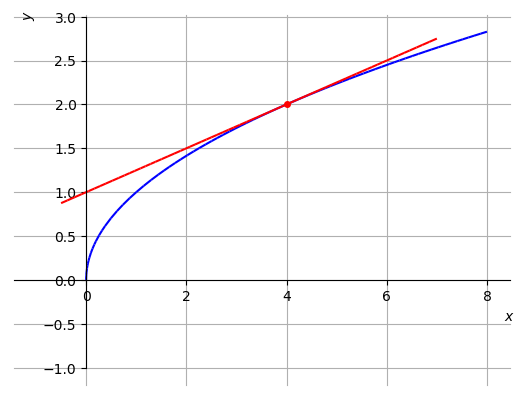
\includegraphics[width=0.7\textwidth]{./cap_deriv/dados/fig_cap_deriv_exeresol_rt_sqrt/fig_cap_deriv_exeresol_rt_sqrt}
    \caption{Esboços do gráfico da função $f$ e da reta tangente no ponto $x_0=4$.}
    \label{fig:cap_deriv_exeresol_rt_sqrt}
  \end{figure}
\end{resol}

\begin{exeresol}
  Considere que a produção em uma empresa tem custo
  \begin{equation}
    c(x) = \sqrt{x}
  \end{equation}
  e rendimento
  \begin{equation}
    r(x) = x^2,
  \end{equation}
  onde $x$ é o número de unidades (em milhões) produzidas. Calcule o lucro marginal da empresa quando $x=1$ mi.
\end{exeresol}
\begin{resol}
  O lucro é
  \begin{equation}
    l(x) = r(x) - c(x).
  \end{equation}
  Desta forma, o lucro marginal no ponto $x_0=1$ é
  \begin{align}
    l'(x_0) &= \lim_{h\to 0} \frac{l(x_0+h)-l(x_0)}{h}\\
            &= \lim_{h\to 0} \frac{r(x_0+h)-c(x_0+h)-(r(x_0)-c(x_0))}{h}\\
            &= \lim_{h\to 0} \frac{r(x_0+h)-r(x_0) - (c(x_0+h)-c(x_0))}{h}\\
            &= \lim_{h\to 0} \frac{r(x_0+h)-r(x_0)}{h} - \lim_{h\to 0} \frac{c(x_0+h)-c(x_0)}{h}\\
            &= r'(x_0) - c'(x_0)\\
            &= 2x_0 - \frac{1}{2\sqrt{x_0}}\\
            &= 2 - \frac{1}{2} = 1,5~\frac{\text{R\$}}{\text{un}}.
  \end{align}
\end{resol}


\subsection*{Exercícios}

\begin{flushright}
  [Vídeo] | [Áudio] | \href{https://phkonzen.github.io/notas/contato.html}{[Contatar]}
\end{flushright}

\begin{exer}
  Calcule as derivadas conforme indicado:
  \begin{enumerate}[a)]
  \item $f(x) = 2$, $f'(-1)$;
  \item $g(x) = 10^6$, $g'(10^8)$;
  \item $h(x) = \ln 2e$, $h'(-\pi)$;
  \end{enumerate}
\end{exer}
\begin{resp}
  a)~$0$; b)~$0$; c)~$0$
\end{resp}

\begin{exer}
  Calcule as derivadas conforme indicado:
  \begin{enumerate}[a)]
  \item $f(x) = 2 + x$, $f'(-1)$;
  \item $g(x) = 10^6 - 2x$, $g'(-3)$;
  \item $h(x) = \ln(2e) + ex$, $h'(10^6)$;
  \end{enumerate}  
\end{exer}
\begin{resp}
  a)~$-1$; b)~$-2$; c)~$e$
\end{resp}

\begin{exer}
  Calcule as derivadas conforme indicado:
  \begin{enumerate}[a)]
  \item $f(x) = x$, $f'(-1)$;
  \item $g(x) = -2x$, $g'(-3)$;
  \item $h(x) = ex$, $h'(10^6)$;
  \end{enumerate}  
\end{exer}
\begin{resp}
  a)~$-1$; b)~$-2$; c)~$e$
\end{resp}

\begin{exer}
  Determine a reta secante ao gráfico de $f(x) = 5-x^2$ pelos pontos $x_0=1$ e $x_1=2$. Então, determine a reta tangente ao gráfico de $f$ no ponto $x_0=1$. Por fim, faça os esboços dos gráficos de $f$, da reta secante e da reta tangente em um mesmo plano cartesiano.
\end{exer}
\begin{resp}
  reta secante: $y = -3x + 7$; reta tangente: $y = -2x + 6$; dica: verifique seus esboços plotando os gráficos no computador
\end{resp}

\begin{exer}
  Assumindo que, em uma empresa, a produção tenha o custo $c(x) = 2\sqrt{x}$ e rendimento $r(x) = \frac{1}{100}x^3$, dados em milhões de reais com $x$ em milhares de unidades. Calcule:
  \begin{enumerate}[a)]
  \item o custo marginal quando $x = 1$;
  \item o rendimento marginal quando $x = 1$;
  \item o lucro marginal quando $x=1$.
  \end{enumerate}
\end{exer}
\begin{resp}
  a)~$1000~\frac{\text{R}\$}{\text{un}}$; b)~$30~\frac{\text{R\$}}{\text{un}}$; c)~$-970~\frac{\text{R\$}}{\text{un}}$.
\end{resp}


\section{Função derivada}\label{cap_deriv_sec_funder}

\begin{flushright}
  [Vídeo] | [Áudio] | \href{https://phkonzen.github.io/notas/contato.html}{[Contatar]}
\end{flushright}

A {\bf derivada} de uma função $f$ em relação à variável $x$ é a função $\displaystyle f' = \frac{\dd f}{\dd x}$ cujo valor em $x$ é
\begin{equation}\label{eq:derivada}
  f'(x) = \lim_{h\to 0} \frac{f(x+h)-f(x)}{h},
\end{equation}
quando este limite existe. Dizemos que $f$ é {\bf derivável} (ou {\bf diferenciável}) em um ponto $x$ de seu domínio, quando o limite dado em \eqref{eq:derivada} existe. Se isso ocorre para todo número real $x$, dizemos que $f$ é derivável em toda parte.

\begin{ex}
  A derivada de $f(x) = x^2$ é
  \begin{align}
    f'(x) &= \lim_{h\to 0} \frac{f(x+h)-f(x)}{h}\\
          &= \lim_{h\to 0} \frac{(x+h)^2 - x^2}{h}\\
          &= \lim_{h\to 0} \frac{x^2+2xh+h^2-x^2}{h}\\
          &= \lim_{h\to 0} 2x+h = 2x.
  \end{align}
  Observamos que este é o caso de uma função derivável em toda parte.A Figura \ref{fig:deriv_ex_ffl_x2}.

  \begin{figure}[H]
    \centering
    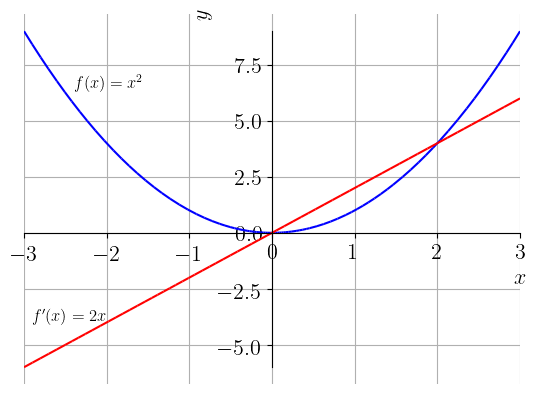
\includegraphics[width=0.7\textwidth]{./cap_deriv/dados/fig_deriv_ex_ffl_x2/fig}
    \caption{Esboços dos gráficos da função $f(x)=x^2$ e de sua derivada $f'(x) = 2x$.}
    \label{fig:deriv_ex_ffl_x2}
  \end{figure}  
  
  \ifispython
  Com o \sympy, podemos usar os seguintes comandos para verificarmos este resultado:
  \begin{lstlisting}
    from sympy import *
    x,h = symbols('x,h')
    f = lambda x: x**2
    limit((f(x+h)-f(x))/h,h,0)
  \end{lstlisting}

  Mais adequadamente, podemos usar o comando:
  \begin{lstlisting}
    diff(x**2,x)
  \end{lstlisting}
  ou, equivalentemente,
  \begin{lstlisting}
    diff(x**2)
  \end{lstlisting}
  para computar a derivada de $x^2$ em relação a $x$.
  \fi
\end{ex}

\begin{obs}
  A derivada à direita (à esquerda) de uma função $f$ em um ponto $x$ é definida por
  \begin{equation}
    f_{\pm}'(x) = \frac{\dd f}{\dd x^{\pm}} = \lim_{h\to 0^\pm} \frac{f(x+h)-f(x)}{h}.
  \end{equation}
  Desta forma, no caso de pontos extremos do domínio de uma função, empregamos a derivada lateral correspondente.
\end{obs}

\begin{ex}\label{ex:deriv_sqrtx}
  Vamos calcular a derivada de $f(x) = \sqrt{x}$. Para $x=0$, só faz sentido calcular a derivada lateral à direta:
  \begin{align}
    f'_{+}(0) &= \lim_{h\to 0^+} \frac{\sqrt{0+h}-\sqrt{0}}{h} \\
              &= \lim_{h\to 0^+} \frac{\sqrt{h}}{h} \\
              &= \lim_{h\to 0^+} \frac{1}{\cancelto{0^+}{\sqrt{h}}} = +\infty.
  \end{align}
  Ou seja, $f(x) = \sqrt{x}$ não é derivável em $x=0$. Agora, para $x> 0$, temos
  \begin{align}
    f'(x) &= \lim_{h\to 0} \frac{\sqrt{x+h}-\sqrt{x}}{h}\\
          &= \lim_{h\to 0} \frac{\sqrt{x+h}-\sqrt{x}}{h}\cdot \frac{\sqrt{x+h}+\sqrt{x}}{\sqrt{x+h}+\sqrt{x}}\\
          &= \lim_{h\to 0} \frac{x+h-x}{h(\sqrt{x+h}+\sqrt{x})}\\
          &= \frac{1}{2\sqrt{x}}.
  \end{align}
  Na Figura \ref{fig:deriv_ex_ffl_sqrtx}, temos os esboços dos gráficos desta função e de sua derivada.

  \begin{figure}[H]
    \centering
    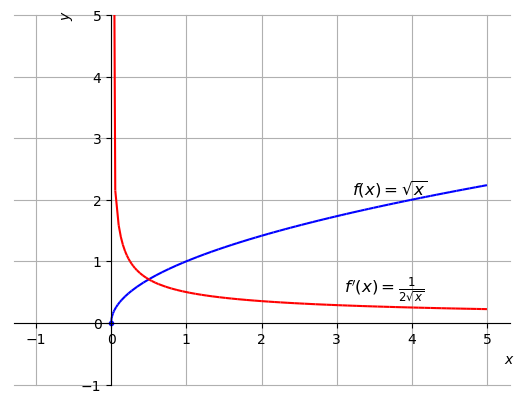
\includegraphics[width=0.7\textwidth]{./cap_deriv/dados/fig_deriv_ex_ffl_sqrtx/fig_deriv_ex_ffl_sqrtx}
    \caption{Esboços dos gráficos da função $f(x)=\sqrt{x}$ e de sua derivada.}
    \label{fig:deriv_ex_ffl_sqrtx}
  \end{figure}

  \ifispython
  No \sympy, a computação de $f'_{+}(0)$ pode ser feita com os comandos\footnote{Por padrão no \sympy, o limite é tomado à direita.}:
  \begin{lstlisting}
    from sympy import *
    h = Symbol('h')
    limit((sqrt(0+h)-sqrt(0))/h,h,0)
  \end{lstlisting}
  E, a derivada de $f(x) = \sqrt{x}$ (nos pontos de diferenciabilidade) pode ser obtida com o comando:
  \begin{lstlisting}
    diff(sqrt(x),x)
  \end{lstlisting}
  \fi
\end{ex}

\begin{ex}\label{ex:deriv_dabs}
  A função valor absoluto é derivável para todo $x\neq 0$ e não é derivável em $x=0$. De fato, para $x<0$ temos
  \begin{align}
    f'(x) &= \lim_{h\to 0} \frac{|x+h|-|x|}{h}\\
          &= \lim_{h\to 0} \frac{-(x+h)+x}{h}\\
          &= \lim_{h\to 0} \frac{h}{h} = 1.
  \end{align}
  Analogamente, para $x>0$ temos
  \begin{align}
    f'(x) &= \lim_{h\to 0} \frac{|x+h|-|x|}{h}\\
          &= \lim_{h\to 0} \frac{x+h-x}{h}\\
          &= \lim_{h\to 0} \frac{h}{h} = 1.
  \end{align}
  Agora, para $x=0$, devemos verificar as derivadas laterais:
  \begin{align}
    f'_+(0) &= \lim_{h\to 0^+} \frac{|h|-|0|}{h} = \lim_{h\to 0^+} \frac{h}{h} = 1,\\
    f'_-(0) &= \lim_{h\to 0^-} \frac{|h|-|0|}{h} = \lim_{h\to 0^-} \frac{-h}{h} = -1.
  \end{align}
  Como as derivadas laterais são diferentes, temos que $y = |x|$ não é derivável em $x=0$. Na figura \ref{fig:deriv_ex_ffl_absx}, temos os esboços dos gráficos de $f(x) = |x|$ e sua derivada
  \begin{equation}\label{eq:deriv_signx}
    f'(x) = \left\{
      \begin{array}[H]{rr}
        -1 &, x<0,\\
        1 &, x> 0
      \end{array}
    \right.
  \end{equation}
  Esta é chamada de {\bf função sinal} e denotada por $\sign(x)$. Ou seja, a função sinal é a derivada da função valor absoluto.

  \begin{figure}[H]
    \centering
    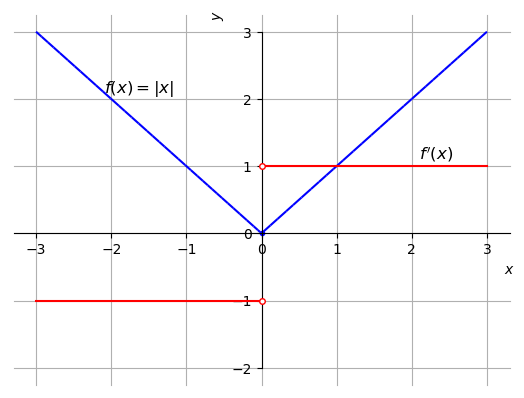
\includegraphics[width=0.7\textwidth]{./cap_deriv/dados/fig_deriv_ex_ffl_absx/fig_deriv_ex_ffl_absx}
    \caption{Esboços dos gráficos da função $f(x)=|x|$ e de sua derivada.}
    \label{fig:deriv_ex_ffl_absx}
  \end{figure}

  \ifispython
  No \sympy, podemos computar a derivada da função valor absoluto com o comando:
  \begin{lstlisting}
    In : from sympy import *
    ...: x = symbols('x', real=True)
    ...: diff(abs(x))
    Out: sign(x)
  \end{lstlisting}
  \fi
\end{ex}

\subsection{Continuidade de uma função derivável}

\begin{flushright}
  [Vídeo] | [Áudio] | \href{https://phkonzen.github.io/notas/contato.html}{[Contatar]}
\end{flushright}

Uma função $y=f(x)$ {\bf derivável} em $x=x_0$ é {\bf contínua} neste ponto. De fato, lembramos que $f$ é contínua em $x=x_0$ quando $x_0$ é um ponto de seu domínio e
\begin{equation}
  \lim_{x\to x_0} f(x) = f(x_0).
\end{equation}
Isto é equivalente a
\begin{equation}
  \lim_{h\to 0} f(x_0+h) = f(x_0)
\end{equation}
ou, ainda,
\begin{equation}
  \lim_{h\to 0} \left[f(x_0+h)-f(x_0)\right] = 0.
\end{equation}
Vamos mostrar que este é o caso quando $f$ é derivável em $x=x_0$. Neste caso, temos
\begin{align}
  \lim_{h\to 0} \left[f(x_0+h)-f(x_0)\right] &= \lim_{h\to 0} \left[f(x_0+h)-f(x_0)\right]\cdot \frac{h}{h} \\
                                             &= \lim_{h\to 0} \left[\cancelto{f'(x_0)}{\frac{f(x_0+h)-f(x_0)}{h}}\right]\cdot h \\
                                             &= \lim_{h\to 0} f'(x_0)\cdot h \\
                                             &= 0.
\end{align}
Ou seja, de fato, se $f$ é derivável em $x=x_0$, então $f$ é contínua em $x=x_0$.

\begin{obs}
  A recíproca não é verdadeira, uma função $f$ ser contínua em um ponto $x=x_0$ não garante que ela seja derivável em $x=x_0$. No Exemplo \ref{ex:deriv_dabs}, vimos que a função valor absoluto $f(x) = |x|$ não derivável em $x=0$, enquanto esta função é contínua (veja, também, o Exemplo \ref{ex:lim_fabs_cont}).
\end{obs}

\subsection{Derivadas de ordens mais altas}

\begin{flushright}
  [Vídeo] | [Áudio] | \href{https://phkonzen.github.io/notas/contato.html}{[Contatar]}
\end{flushright}

A derivada de uma função $y = f(x)$ em relação a $x$ é a função $y = f'(x)$. Quando esta é diferenciável, podemos calcular a derivada da derivada. Esta é conhecida como a {\bf segunda derivada} de $f$, denotamos
\begin{equation}
  f''(x) := (f'(x))' ~ \text{ou} ~ \frac{\dd^2}{\dd x^2}f(x) = \frac{\dd}{\dd x}\left(\frac{\dd}{\dd x}f(x)\right).
\end{equation}

\begin{ex}\label{ex:deriv_fll}
  Seja $f(x) = x^3$. Então, a primeira derivada de $f$ é
  \begin{align}
    f'(x) &= \lim_{h\to 0} \frac{f(x+h)-f(x)}{h} \\
          &= \lim_{h\to 0} \frac{(x+h)^3-x^3}{h}\\
          &= \lim_{h\to 0} \frac{x^3+3x^2h+3xh^2+h^3-x^3}{h}\\
          &= \lim_{h\to 0} 3x^2+\cancelto{0}{3xh}+\cancelto{0}{h^2} = 3x^2.
  \end{align}
  De posse da primeira derivada $f'(x) = 3x^2$, podemos calcular a segunda derivada de $f$, como segue:
  \begin{align}
    f''(x) &= [f'(x)]' \\
           &= \lim_{h\to 0} \frac{f'(x+h)-f'(x)}{h} \\
           &= \lim_{h\to 0} \frac{3(x+h)^2-3x^2}{h} \\
           &= \lim_{h\to 0} \frac{3x^2+6xh+h^2-3x^2}{h} \\
           &= \lim_{h\to 0} 6x+\cancelto{0}{h} = 6x,
  \end{align}
  i.e. $f''(x) = 6x$.

  \ifispython
  No \sympy, podemos computar a segunda derivada da função com o comando:
  \begin{lstlisting}
    In : from sympy import *
    ...: x = symbols('x')
    ...: diff(x**3,x,2)
    Out: 6*x
  \end{lstlisting}
  \fi  
\end{ex}

Generalizando, quando existe, a $n$-ésima derivada de uma função $y = f(x)$, $n\geq 1$, é recursivamente definida (e denotada) por
\begin{equation}
  f^{(n)}(x) := [f^{(n-1)}]' ~ \text{ou} ~ \frac{\dd^n}{\dd x^n}f(x) := \frac{\dd}{\dd x}\left[\frac{\dd^{n-1}}{\dd x^{n-1}}f(x)\right],
\end{equation}
com $f^{(3)}\equiv f'''$, $f^{(2)}\equiv f''$, $f^{(1)}\equiv f'$ e $f^{(0)}\equiv f$.

\begin{ex}
  A terceira derivada de $f(x) = x^3$ em relação a $x$ é $f'''(x) = [f''(x)]'$. No exemplo anterior (Exemplo \ref{ex:deriv_fll}), calculamos $f''(x) = 6x$. Logo,
    \begin{align}
      f'''(x) &= [6x]' \\
              &= \lim_{h\to 0} \frac{6(x+h)-6x}{h} \\
              &= \lim_{h\to 0} 6 = 6.
    \end{align}

    A quarta derivada de $f(x) = x^3$ em relação a $x$ é $f^{(4)}(x) \equiv 0$, bem como $f^{(5)}(x) \equiv 0$. Verifique!

    \ifispython
    No \sympy, podemos computar a terceira derivada da função com o comando:
    \begin{lstlisting}
      In : from sympy import *
      ...: x = symbols('x')
      ...: diff(x**3,x,3)
      Out: 6
    \end{lstlisting}
  \fi  
\end{ex}


\subsection*{Exercícios resolvidos}

\begin{flushright}
  [Vídeo] | [Áudio] | \href{https://phkonzen.github.io/notas/contato.html}{[Contatar]}
\end{flushright}

\begin{exeresol}
  Calcule a derivada da função $f(x) = x^2 + 2x + 1$ em relação a $x$.
\end{exeresol}
\begin{resol}
  Por definição da derivada, temos
  \begin{align}
    f'(x) &= \lim_{h\to 0} \frac{f(x+h)-f(x)}{h}\\
          &= \lim_{h\to 0} \frac{(x+h)^2 + 2(x+h) + 1 - (x^2+2x+1)}{h}\\
          &= \lim_{h\to 0} \frac{x^2+2xh+h^2+2x+2h+1-x^2-2x-1}{h}\\
          &= \lim_{h\to 0} \frac{2xh+h^2+2h}{h}\\
          &= \lim_{h\to 0} 2x+h+2 = 2x+2.
  \end{align}
\end{resol}

\begin{exeresol}
  Determine os pontos de diferenciabilidade da função $f(x) = |x-1|$.
\end{exeresol}
\begin{resol}
  O gráfico da função $f(x) = |x-1|$ tem um bico no ponto $x=1$ (verifique!). Para valores de $x<1$, temos
  \begin{align}
    f'(x) &= \lim_{h\to 0} \frac{f(x+h) - f(x)}{h}\\
          &= \lim_{h\to 0} \frac{|\overbrace{x+h-1}^{<0}| - |\overbrace{x-1}^{<0}|}{h}\\
          &= \lim_{h\to 0} \frac{-x-h+1+x-1}{h}\\
          &= \lim_{h\to 0} \frac{-h}{h} = -1.
  \end{align}
  Para valores de $x > 1$, temos
  \begin{align}
    f'(x) &= \lim_{h\to 0} \frac{f(x+h) - f(x)}{h}\\
          &= \lim_{h\to 0} \frac{|\overbrace{x+h-1}^{>0}| - |\overbrace{x-1}^{>0}|}{h}\\
          &= \lim_{h\to 0} \frac{x+h-1-x+1}{h}\\
          &= \lim_{h\to 0} \frac{h}{h} = 1.
  \end{align}
  Ou seja, temos que $f(x) = |x-1|$ é diferenciável para $x\neq 1$. Agora, para $x=1$, temos
  \begin{align}
    f'_{-}(x) &= \lim_{h\to 0^{-}} \frac{f(1+h) - f(1)}{h}\\
              &= \lim_{h\to 0^{-}} \frac{|\overbrace{h}^{<0}| - |1-1|}{h}\\
              &= \lim_{h\to 0^{-}} \frac{-h}{h} = -1\\
    f'_{+}(x) &= \lim_{h\to 0^{+}} \frac{f(1+h) - f(1)}{h}\\
          &= \lim_{h\to 0^{+}} \frac{|\overbrace{h}^{>0}| - |1-1|}{h}\\
              &= \lim_{h\to 0^{+}} \frac{h}{h} = 1\\
  \end{align}
  Como $f'_{-}(1)\neq f'_{+}(1)$, temos que $\nexists f'(1)$. Concluímos que $f(x) = |x-1|$ é diferenciável nos pontos $\mathbb{R}\setminus\{1\}$. 
\end{resol}

\begin{exeresol}
  Calcule a segunda derivada em relação a $x$ da função
  \begin{equation}
    f(x) = x - x^2.
  \end{equation}
\end{exeresol}
\begin{resol}
  Começamos calculando a primeira derivada da função:
  \begin{align}
    f'(x) &= \lim_{h\to 0} \frac{f(x+h)-f(x)}{h} \\
          &= \lim_{h\to 0} \frac{(x+h)-(x+h)^2-(x-x^2)}{h} \\
          &= \lim_{h\to 0} \frac{x+h-x^2-2xh-h^2-x+x^2}{h} \\
          &= \lim_{h\to 0} 1-2x-\cancelto{0}{h} = 1 - 2x.
  \end{align}
  Então, calculamos a segunda derivada como segue
  \begin{align}
    f''(x) &= [f'(x)]' \\
           &= \lim_{h\to 0} \frac{f'(x+h)-f'(x)}{h} \\
           &= \lim_{h\to 0} \frac{1-2(x+h)-(1-2x)}{h} \\
           &= \lim_{h\to 0} -2 = -2.
  \end{align}
\end{resol}

\subsection*{Exercícios}

\begin{flushright}
  [Vídeo] | [Áudio] | \href{https://phkonzen.github.io/notas/contato.html}{[Contatar]}
\end{flushright}

\begin{exer}
  Calcule a derivada em relação a $x$ de cada uma das seguintes funções:
  \begin{enumerate}[a)]
  \item $f(x) = 2$
  \item $g(x) = -3$
  \item $h(x) = \sqrt{e}$
  \end{enumerate}
\end{exer}
\begin{resp}
  a)~$0$; b)~$0$; c)~$0$
\end{resp}

\begin{exer}
  Calcule a derivada em relação a $x$ de cada uma das seguintes funções:
  \begin{enumerate}[a)]
  \item $f(x) = 2x$
  \item $g(x) = -3x$
  \item $h(x) = \sqrt{e}x$
  \end{enumerate}
\end{exer}
\begin{resp}
  a)~$2$; b)~$-3$; c)~$\sqrt{e}$
\end{resp}

\begin{exer}
  Calcule a derivada em relação a $x$ da função
  \begin{equation}
    f(x) = x^2 - 2x + 1.
  \end{equation}
\end{exer}
\begin{resp}
  $f'(x) = 2x - 2$
\end{resp}

\begin{exer}
  Determine os pontos de diferenciabilidade da função $f(x) = \sqrt{x-1}$.
\end{exer}
\begin{resp}
  $(1, \infty)$
\end{resp}

\begin{exer}
  Considerando
  \begin{equation}
    f(x) = x^2-x^3,
  \end{equation}
  calcule:
  \begin{enumerate}[a)]
  \item $f'(x)$
  \item $f''(x)$
  \item $f'''(x)$
  \item $f^{(4)}$
  \item $f^{(1001)}(x)$
  \end{enumerate}
\end{exer}
\begin{resp}
  a)~$2x-3x^2$; b)~$2-6x$; c)~$-6$; d)~$0$; e)~$0$
\end{resp}

\section{Regras básicas de derivação}\label{cap_deriv_sec_regras}

\begin{flushright}
  [Vídeo] | [Áudio] | \href{https://phkonzen.github.io/notas/contato.html}{[Contatar]}
\end{flushright}

Nesta seção, vamos estudar sobre algumas regras fundamentais para o cálculo da derivada de funções. Começaremos pelas derivadas de função constante, de função potência e de função exponencial. Em seguida, passamos a derivadas da soma, multiplicação e quociente de funções.

\subsection{Derivadas de função constante e função potência}

\begin{flushright}
  [Vídeo] | [Áudio] | \href{https://phkonzen.github.io/notas/contato.html}{[Contatar]}
\end{flushright}

Vejamos as derivadas da função constante e da função potência.
\begin{itemize}
\item $(k)' = 0$, onde $k$ é uma constante.

  De fato, para $f(x) \equiv k$ temos
  \begin{align}
    f'(x) &= \lim_{h\to 0} \frac{f(x+h)-f(x)}{h}\\
          &= \lim_{h\to 0} \frac{k-k}{h} \\
          &= \lim_{h\to 0} 0 = 0.
  \end{align}

\item $\pmb{(x)' = 1}$.

  De fato, para a função identidade $f(x) = x$ temos
  \begin{align}
    f'(x) &= \lim_{h\to 0} \frac{f(x+h)-f(x)}{h}\\
          &= \lim_{h\to 0} \frac{x+h-x}{h}\\
          &= \lim_{h\to 0} \frac{h}{h} = 1.\\
  \end{align}

\item $\pmb{(x^n)' = nx^{n-1}}$, para $n > 1$ inteiro positivo.

  De fato, para $f(x) = x^n$ temos
  \begin{align}
    f'(x) &= \lim_{h\to 0} \frac{f(x+h)-f(x)}{h}\\
          &= \lim_{h\to 0} \frac{(x+h)^n-x^n}{h} \\
          &= \lim_{h\to 0} \frac{x^n+nx^{n-1}h+\frac{n(n-1)}{2}x^{n-2}h^2 + \cdots +h^n-x^n}{h}\\
          &= \lim_{h\to 0} nx^{n-1}+\frac{n(n-1)}{2}x^{n-2}h+\cdots+h^{n-1}\\
          &= nx^{n-1}.
  \end{align}
\end{itemize}

\ifispython
No \sympy, podemos usar os seguintes comandos para obtermos as regras de derivação acima:
\begin{lstlisting}
  from sympy import *
  # (k)' = 0
  k = Symbol('k', real=True, constant=True)
  diff(k,x)

  # (x)' = 1
  x = Symbols('x')
  diff(x,x)

  # (x^n)' = nx^(n-1)
  n = Symbols('n',integer=True, positive=True)
  diff(x**n,x)
\end{lstlisting}
\fi

\begin{ex}
  Vejamos os seguintes casos:
  \begin{enumerate}[a)]
  \item $(-1)' = 0$.
  \item $(\sqrt{2})' = 0$.
  \item $(x^3)' = 3x^2$.
  \item $(x^{11})' = 11x^{10}$.
  \end{enumerate}
\end{ex}

\subsection{Derivada de função exponencial}

\begin{flushright}
  [Vídeo] | [Áudio] | \href{https://phkonzen.github.io/notas/contato.html}{[Contatar]}
\end{flushright}

Vejamos o cálculo da derivada de função exponencial.

\begin{itemize}
\item $\pmb{(a^x)' = a^x\ln a}$, para $a>0$ e $a\neq 1$.
  
  De fato, tomando $f(x) = a^x$, $a>0$ e $a\neq 1$ temos
  \begin{align}
    f'(x) &= \lim_{h\to 0} \frac{f(x+h)-f(x)}{h}\\
          &= \lim_{h\to 0} \frac{a^{x+h}-a^x}{h} \\
          &= \lim_{h\to 0} \frac{a^xa^h-a^x}{h} \\
          &= a^x \lim_{h\to 0} \frac{a^h-1}{h}
  \end{align}
  Pode-se mostrar que\footnote{Pode-se mostrar isso a partir da definição integral da função logaritmo.}
  \begin{equation}
    \lim_{h\to 0} \frac{a^h-1}{h} = \ln a.
  \end{equation}
  Desta forma, temos
  \begin{equation}
    f'(x) = a^x\ln a = (a^x)'.
  \end{equation}

\item $\pmb{(e^x)' = e^x}$.

  De fato, $(a^x)' = a^x\ln a$, para $a>0$ e $a\neq 1$. Tomando $a = e$, temos
  \begin{equation}
    (e^x)' = e^x\underbrace{\ln e}_{=1} = e^x.
  \end{equation}
\end{itemize}

\ifispython
No \sympy, podemos usar os seguintes comandos para computarmos as derivadas acima:
\begin{lstlisting}
  from sympy import *
  a = Symbol('a', real=True)
  # (a^x)'
  diff(a**x,x)
  
  # (e^x)'
  diff(E**x,x)
\end{lstlisting}
\fi


\begin{ex}
Vejamos os seguintes casos:
\begin{enumerate}[a)]
\item $(2^x)' = 2^x\ln 2$.
\item $(e^x)' = e^x$.
\end{enumerate}

\ifispython
No \sympy, podemos usar os seguintes comandos para computarmos as derivadas acima:
\begin{verbatim}
# a)
diff(2**x,x)
# b)
diff(E**x,x)
\end{verbatim}
\fi
\end{ex}

\subsection{Regras da multiplicação por constante e da soma}\label{subsec:deriv_rmcs}

\begin{flushright}
  [Vídeo] | [Áudio] | \href{https://phkonzen.github.io/notas/contato.html}{[Contatar]}
\end{flushright}

Sejam $k$ um número real, $u = u(x)$ e $v = v(x)$ funções deriváveis. Temos as seguintes regras básicas de derivação:
\begin{itemize}
\item $\pmb{(k\cdot u)' = k\cdot u'}$.

  De fato, pela definição da derivada temos
  \begin{align}
    (k\cdot u)'(x) &= \lim_{h\to 0} \frac{k\cdot u(x+h)-k\cdot u(x)}{h} \\
                   &= \lim_{h\to 0} k\cdot \left(\frac{u(x+h)-u(x)}{h}\right) \\
                   &= k\cdot \lim_{h\to 0} \cancelto{u'}{\frac{u(x+h)-u(x)}{h}} \\
                   &= k\cdot u'.
  \end{align}
  
  \ifispython
  No \sympy, podemos usar os seguintes comandos para obtermos esta regra de derivação:
  \begin{lstlisting}
    from sympy import *
    k = Symbol('k', real=True)
    u = Function('u', real=True)
    diff(k*u(x),x)
  \end{lstlisting}
  \fi

\item $\pmb{(u\pm v)' = u'\pm v'}$.

  De fato, temos
  \begin{align}
    (u + v)'(x) &= \lim_{h\to 0} \frac{(u + v)(x+h)-(u + v)(x)}{h}\\
                &= \lim_{h\to 0} \frac{u(x+h)+v(x+h)-[u(x)+v(x)]}{h}\\
                &= \lim_{h\to 0} \left[\cancelto{u'}{\frac{u(x+h)-u(x)}{h}} \right. \\
                &+ \left. \cancelto{v'}{\frac{v(x+h)-v(x)}{h}}\right]\\
                &= u'(x) + v'(x).
  \end{align}

  Também, como $(-v)' = (-1\cdot v)' = -1\cdot v' = -v'$, temos
  \begin{equation}
    (u-v)' = [u+(-v)]' = u' + (-v)' = u' - v'.
  \end{equation}
  
  \ifispython
  No \sympy, podemos usar os seguintes comandos para obtermos a regra de derivação para soma:
  \begin{lstlisting}
    from sympy import *
    u = Function('u', real=True)
    v = Function('v', real=True)
    diff(u(x)+v(x),x)
  \end{lstlisting}
  \fi
\end{itemize}

\begin{ex}
  Vejamos os seguintes casos:
  \begin{enumerate}[a)]
  \item $f(x) = 2x$.

    Para calcularmos $f'$, podemos identificar $f = k\cdot u$, com $k=2$ e $u(x) = x$. Então, usando a regra da multiplicação por constante $(ku)' = ku'$, temos
    \begin{equation}
      f'(x) = (2x)' = 2(x') = 2\cdot 1 = 2.
    \end{equation}

  \ifispython
  No \sympy, podemos computar esta derivada com o comando:
  \begin{lstlisting}
    from sympy import *
    x = Symbol('x')
    diff(2*x,x)
  \end{lstlisting}
  \fi
    

  \item $f(x) = 2x + 3$.

    Observamos que $f = u + v$, com $u(x) = 2x$ e $v(x)\equiv 3$. Então, da regra da soma $(u+v)' = u' + v'$, temos
    \begin{equation}
      f'(x) = (2x + 3)' = (2x)' + (3)' = 2 + 0 = 2.
    \end{equation}

    \ifispython
    No \sympy, podemos computar esta derivada com o comando:
    \begin{lstlisting}
      from sympy import *
      x = Symbols('x')
      diff(2*x+3,x)
    \end{lstlisting}
    \fi

  \item $f(x) = e^x - x^2$.

    Observamos que $f = u-v$, com $u(x) = e^x$ e $v(x)= x^2$. Usando a regra da subtração $(u-v)' = u' - v'$ temos
    \begin{equation}
      f'(x) = (e^x - x^2)' = (e^x)' - (x^2)' = e^x - 2x.
    \end{equation}

    \ifispython
    No \sympy, podemos computar esta derivada com o comando:
    \begin{lstlisting}
      from sympy import *
      x = Symbols('x')
      diff(exp(x)-x**2,x)
    \end{lstlisting}
    \fi
  \end{enumerate}
\end{ex}

\subsection{Regras do produto e do quociente}

\begin{flushright}
  [Vídeo] | [Áudio] | \href{https://phkonzen.github.io/notas/contato.html}{[Contatar]}
\end{flushright}

Sejam $y = u(x)$ e $y = v(x)$ funções deriváveis. Então:
\begin{itemize}
\item $\pmb{(u\cdot v)' = u'\cdot v+u\cdot v'}$.

  De fato, da definição da derivada temos
  \begin{align}
    (uv)'(x) &= \lim_{h\to 0} \frac{(uv)(x+h)-(uv)(x)}{h}\\
             &= \lim_{h\to 0} \frac{u(x+h)v(x+h)-u(x)v(x)}{h}\\
             &= \lim_{h\to 0} \left[\frac{u(x+h)v(x+h)-u(x)v(x+h)}{h}\right.\\
             &\qquad\quad+ \left.\frac{u(x)v(x+h)-u(x)v(x)}{h}\right]\\
             &= \lim_{h\to 0} \frac{u(x+h)-u(x)}{h}v(v+h) \\
             &+ \lim_{h\to 0} u(x)\frac{v(x+h)-v(x)}{h}\\
             &= u'(x)v(x) + u(x)v'(x).
  \end{align}
  
  \ifispython
  No \sympy, podemos usar os seguintes comandos para obtermos tal regra de derivação:
  \begin{lstlisting}
    u = Function('u', real=True)
    v = Function('v', real=True)
    diff(u(x)*v(x), x)
  \end{lstlisting}
  \fi
  
\item $\displaystyle\pmb{\left(\frac{u}{v}\right)' = \frac{u'v-uv'}{v^2}}$, no caso de $v(x)\neq 0$.

  De fato, da definição de derivada temos
  \begin{align}
    \left(\frac{u}{v}\right)'(x) &= \lim_{h\to 0} \frac{\left(\frac{u}{v}\right)(x+h)-\left(\frac{u}{v}\right)(x)}{h} \\
                                 &= \lim_{h\to 0} \frac{\frac{u(x+h)v(x)-u(x)v(x+h)}{v(x+h)v(x)}}{h}\\
                                 &= \lim_{h\to 0} \left[\frac{u(x+h)v(x)-u(x)v(x)}{h}\right. \\
                                 &\qquad\quad - \left.\frac{u(x)v(x+h)-u(x)v(x)}{h}\right]\frac{1}{v(x)v(x+h)}\\
                                 &= \left[\lim_{h\to 0} \cancelto{u'(x)v(x)}{\frac{u(x+h)-u(x)}{h}v(x)}\right. \\
                                 &\left. - \lim_{h\to 0} \cancelto{u(x)v'(x)}{u(x)\frac{v(x+h)-v(x)}{h}}\right]\lim_{h\to 0} \cancelto{\frac{1}{v^2(x)}}{\frac{1}{v(x)v(x+h)}}\\
                                 &= \frac{u'(x)v(x)-u(x)v'(x)}{v^2(x)}.
  \end{align}
  
  \ifispython
  No \sympy, podemos usar os seguintes comandos para obtermos tal regra de derivação:
  \begin{lstlisting}
    from sympy import *
    x = Symbol('x')
    u = Function('u', real=True)
    v = Function('v', real=True)
    simplify(diff(u(x)/v(x),x))
\end{lstlisting}
  \fi
\end{itemize}

\begin{ex}
  Vamos calcular a derivada em relação a $x$ da função $f(x) = x^2(x-1)$ de duas formas.
  \begin{enumerate}[1.]
  \item Por expansão da expressão e utilização da regra da subtração.
    \begin{align}
      f'(x) &= [x^2(x-1)]'\\
            &= (x^3-x^2)' \\
            &= \overbrace{(x^3)'-(x^2)'}^{(u-v)'=u'-v'}\\
            &= 3x^2-2x,\quad\quad(x^n)' = nx^{n-1}.
    \end{align}
  \item Utilizando a regra do produto.

    Observamos que $f = u\cdot v$, com $u(x) = x^2$ e $v(x) = x-1$. Então, da regra do produto $(uv)' = u'v + uv'$, com $u'(x) = 2x$ e $v'(x) = 1$, temos
    \begin{align}
      f'(x) &= [\overbrace{x^2}^{u}\overbrace{(x-1)}^{v}]'\\
            &= \overbrace{2x\cdot (x-1)}^{u'\cdot v} + \overbrace{x^2\cdot 1}^{u\cdot v'}\\
            &= 2x^2 - 2x + x^2\\
            &= 3x^2 - 2x.
    \end{align}
  \end{enumerate}
\end{ex}

\begin{ex}\label{ex:deriv_x-2}
  Vamos calcular a derivada em relação a $x$ de $f(x) = 1/x^2$ para $x\neq 0$. Observamos que $f = (u/v)$ com $u(x) \equiv 1$ e $v(x) = x^2$. Tendo em vista que $u'(x) \equiv 0$ e $v'(x) = 2x$, temos da regra do quociente que
  \begin{align}
    f'(x) &= \left(\frac{1}{x^2}\right)' \\
          &= \frac{0\cdot x^2 - 1\cdot 2x}{(x^2)^2},\quad\quad\left[\left(\frac{u}{v}\right)' = \frac{u'v-uv'}{v^2}\right]\\
          &= -\frac{2x}{x^4} = -\frac{2}{x^3}\\
          &= -2x^{-3}.
  \end{align}
\end{ex}

\begin{obs}
  Com abuso de linguagem, temos
  \begin{equation}
    \pmb{(x^n)' = nx^{n-1}},
  \end{equation}
  com $n$ inteiro. No caso de $n=1$, temos $(x)' \equiv 1$. No caso de $n <= 0$, devemos ter $x\neq 0$\footnote{Devido a indeterminação de $0^0$ e a inexistência de $0^n$ com $n$ negativo}. Mai ainda, a regra também vale para $n=1/2$, veja o Exemplo \ref{ex:deriv_sqrtx}. 
\end{obs}

\begin{ex}
  Voltando ao exemplo anterior (Exemplo \ref{ex:deriv_x-2}), temos
  \begin{equation}
    \left(\frac{1}{x^2}\right)' = \overbrace{(x^{-2})'}^{(x^n)'} = \overbrace{-2x^{-2-1}}^{nx^{n-1}} = -2x^{-3}.
  \end{equation}
\end{ex}

\begin{ex}
  Vamos calcular a derivada em relação a $x$ de $f(x) = xe^x$. Usando a regra do produto $(uv)' = u'v + uv'$ com $u(x) = x$ e $v(x) = e^x$, temos
  \begin{align}
    f'(x) &= \overbrace{(xe^x)'}^{(uv)'}\\
          &= \overbrace{1\cdot e^x}^{u'\cdot v} + \overbrace{x\cdot e^x}^{u\cdot v'}\\
          &= (x + 1)e^x.
  \end{align}
\end{ex}

\subsection{Tabela de derivadas}

\begin{flushright}
  [Vídeo] | [Áudio] | \href{https://phkonzen.github.io/notas/contato.html}{[Contatar]}
\end{flushright}

\begin{align}
  &(ku)' = ku' && (u\pm v)' = u' \pm v'\\
  &(uv)' = u'v + uv' && \left(\frac{u}{v}\right)' = \frac{u'v - uv'}{v^2} \\
  &(k)' = 0 && (x^n)' = nx^{n-1}\\
  &(a^x)' = a^x\ln a && (e^x)' = e^x \\
\end{align}


\subsection*{Exercícios resolvidos}

\begin{flushright}
  [Vídeo] | [Áudio] | \href{https://phkonzen.github.io/notas/contato.html}{[Contatar]}
\end{flushright}

\begin{exeresol}
  Calcule a derivada em relação a $x$ da função
  \begin{equation}
    f(x) = (x^2+x)(1 + x^3) - 2x^2.
  \end{equation}
\end{exeresol}
\begin{resol}
  \begin{align}
    f'(x) &= \overbrace{\left[(x^2+x)(1 + x^3) - 2x^2\right]'}^{(u-v)'} \\
          &= \overbrace{\left[(x^2+x)(1 + x^3)\right]'}^{(uv)'} - \overbrace{(2x^2)'}^{(ku)'} \\
          &= (x^2+x)'(1+x^3) + (x^2+x)(1+x^3)' - 2(x^2)'\\
          &= (2x+1)(1+x^3) + (x^2+x)3x^2 - 4x\\
          &= 2x+2x^4+1+x^3+3x^4+3x^3-4x\\
          &= 5x^4+4x^3-2x+1.
  \end{align}
  
  \ifispython
  Com o \sympy, podemos computar esta derivada com os seguintes comandos:
  \begin{lstlisting}
    from sympy import *
    x = Symbol('x')
    d = diff((x**2+x)*(1+x**3)-2x^2,x)
    simplify(d)
  \end{lstlisting}
  \fi
\end{resol}

\begin{exeresol}
  Calcule
  \begin{equation}
    \frac{\dd}{\dd x}\left(\frac{x^2+x}{1-x^3}\right).
  \end{equation}
\end{exeresol}
\begin{resol}
  Da regra de derivação do quociente, temos
  \begin{align}
    \frac{\dd}{\dd x}\left(\frac{x^2+x}{1-x^3}\right) &= \frac{(x^2+x)'(1-x^3)-(x^2+x)(1-x^3)'}{(1-x^3)^2}\\
                                                      &= \frac{(2x+1)(1-x^3)+(x^2+x)3x^2}{1-2x^3+x^6} \\
                                                      &= \frac{2x-2x^4+1-x^3+3x^4+3x^3}{1-2x^3+x^6} \\
                                                      &= \frac{x^4+2x^3+2x+1}{x^6-2x^3+1}
  \end{align}
  
  \ifispython
  Com o \sympy, podemos computar esta derivada com os seguintes comandos:
  \begin{lstlisting}
    from sympy import *
    x = Symbol('x')
    d = diff((x**2+x)/(1-x**3),x)
    simplify(d)
  \end{lstlisting}
  \fi
\end{resol}

\begin{exeresol}
  Encontre a equação da reta tangente ao gráfico de $f(x) = xe^{-x}$ no ponto $x=1$.
\end{exeresol}
\begin{resol}
  A equação da reta tangente ao gráfico de uma função $f$ no ponto $x=x_0$ é
  \begin{equation}
    y = f'(x_0)(x-x_0)+f(x_0).
  \end{equation}
  No caso, temos $f(x)=xe^{-x}$ e $x_0=1$. Calculamos
  \begin{align}
    f'(x) &= [xe^{-x}]' = \left[\frac{x}{e^x}\right] \\
          &= \frac{(x)'e^x-x(e^x)'}{(e^x)^2} \\
          &= \frac{e^x-xe^x}{e^{2x}} \\
          &= \frac{(1-x)e^x}{e^{2x}} \\
          &= (1-x)e^xe^{-2x} = (1-x)e^{-x}.
  \end{align}
  Logo, a equação da reta tangente é
  \begin{gather}
    y = f'(1)(x-1)+f(1) \\
    y = 0\cdot (x-1) + e^{-1} \\
    y = \frac{1}{e}.
  \end{gather}
  Na Figura \ref{fig:deriv_exeresol_rt_xe-x}, temos os esboços dos gráfico da função $f$ e sua reta tangente no ponto $x=1$.

  \begin{figure}[H]
    \centering
    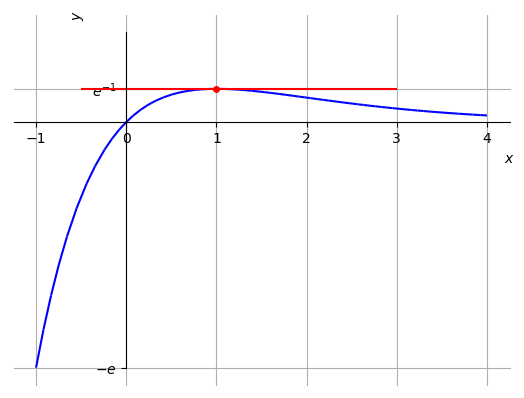
\includegraphics[width=0.7\textwidth]{./cap_deriv/dados/fig_deriv_exeresol_rt_xe-x/fig_deriv_exeresol_rt_xe-x}
    \caption{Esboço da reta tangente ao gráfico de $f(x)=xe^{-x}$ no ponto $x=1$.}
    \label{fig:deriv_exeresol_rt_xe-x}
  \end{figure}

  \ifispython
  Com o \sympy, podemos computar a expressão desta reta tangente com os seguintes comandos:
  \begin{lstlisting}
    from sympy import *
    x = Symbol('x')
    f = x*exp(-x)
    x0 = 1
    fl = diff(f,x)
    # y = 
    fl.subs(x,1)*(x-1)+f.subs(x,1)
  \end{lstlisting}
  \fi
\end{resol}

\subsection*{Exercícios}

\begin{flushright}
  [Vídeo] | [Áudio] | \href{https://phkonzen.github.io/notas/contato.html}{[Contatar]}
\end{flushright}

\begin{exer}
  Calcule a derivada em relação a $x$ das seguintes funções:
  \begin{enumerate}[a)]
  \item $f(x) = 2 - 5x^3$ \\
  \item $g(x) = (2x-1)(2-4x^2)$
  \item $h(x) = \frac{2-4x^2}{2x-1}$
  \end{enumerate}
\end{exer}
\begin{resp}
  a)~$f'(x) = -15x^2$; b)~$g'(x)=- 24 x^{2} + 8 x + 4$; c)~$\displaystyle h'(x) = \\frac{4 \\left(2 x^{2} - 2 x \\left(2 x - 1\\right) - 1\\right)}{\\left(2 x - 1\\right)^{2}}$
\end{resp}

\begin{ex}
  Calcule a derivada em relação a $x$ das seguintes funções:
  \begin{enumerate}[a)]
  \item $f(x) = xe^x$
  \item $g(x) = xe^{2x}$
  \item $g(x) = xe^{-2x}$
  \end{enumerate}
\end{ex}
\begin{resp}
  a)~$f'(x) = (1+x)e^x$; b)~$g'(x) = (1+2x)e^{2x}$; c)~$h'(x) = (1-2x)e^{-2x}$
\end{resp}

\begin{ex}
  Calcule a derivada em relação a $x$ das seguintes funções:
  \begin{enumerate}[a)]
  \item $f(x) = \ln x^2$
  \item $g(x) = x\ln x^2$
  \item $g(x) = x\ln x^2e^x$
  \end{enumerate}
\end{ex}
\begin{resp}
  a)~$f'(x) = 2/x$; b)~$g'(x) = \ln x^2 + 2$; c)~$h'(x) = 2+2x+\ln x^2$
\end{resp}

\begin{ex}
  Encontre a equação da reta tangente ao gráfico de $f(x) = \ln x$ no ponto $x=1$.
\end{ex}
\begin{resp}
  $y = x-1$
\end{resp}

\section{Derivadas de funções trigonométricas}\label{cap_deriv_sec_trigo}

\begin{flushright}
  [Vídeo] | [Áudio] | \href{https://phkonzen.github.io/notas/contato.html}{[Contatar]}
\end{flushright}

Começamos pela derivada da função seno. Pela definição da derivada, temos
\begin{align}
  \sen' x &= \lim_{h\to 0} \frac{\sen(x+h) - \sen x}{h} \\
            &= \lim_{h\to 0} \frac{\sen(x)\cos(h)+\cos(x)\sen(h) - \sen x}{h} \\
            &= \lim_{h\to 0} \sen(x)\frac{\cos(h) - 1}{h} + \cos(x)\frac{\sen h}{h}\\
            &= \sen(x) \lim_{h\to 0} \frac{\cos(h)-1}{h} + \cos(x)\lim_{h\to 0} \frac{\sen h}{h}.
\end{align}
Usando do Teorema do confronto para limites de funções, podemos mostrar que\footnote{Veja a Seção \ref{sec:lim_senx_x}.}
\begin{equation}
  \lim_{h\to 0} \frac{\sen h}{h} = 1\quad\text{e}\quad\lim_{h\to 0} \frac{\cos(h) - 1}{h} = 0.
\end{equation}
Logo, temos
\begin{equation}
  \pmb{\sen' x = \cos x}.
\end{equation}

De forma similar, temos
\begin{align}
  \cos' x &= \lim_{h\to 0} \frac{\cos(x+h) - \cos x}{h} \\
            &= \lim_{h\to 0} \frac{\cos(x)\cos(h)-\sen(x)\sen(h) - \cos x}{h} \\
            &= \lim_{h\to 0} \cos(x)\frac{\cos(h) - 1}{h} - \sen(x)\frac{\sen h}{h}\\
            &= \cos(x) \lim_{h\to 0} \cancelto{0}{\frac{\cos(h)-1}{h}} - \sen(x)\lim_{h\to 0} \cancelto{0}{\frac{\sen h}{h}}.
\end{align}
Ou seja,
\begin{equation}
  \pmb{\cos' x = -\sen x}.
\end{equation}

\begin{ex}
  A derivada de $f(x) = \sen^2 x + \cos^2 x$ é
  \begin{align}
    f'(x) &= (\sen^2x + \cos^2 x)' \\
          &= (\sen^2 x)' + (\cos^2 x)' \\
          &= (\sen x\cdot \sen x)' + (\cos x\cdot \cos x)' \\
          &= \cos x\cdot \sen x + \sen x\cdot\cos x -\sen x\cdot \cos x - \cos x\cdot\sen x\\
          &= 0,
  \end{align}
  conforme esperado.

  \ifispython
  Com o \sympy, podemos computar esta derivada com o seguinte comando:
\begin{lstlisting}
    from sympy import *
    x = Symbol('x')
    diff(sin(x)**2+cos(x)**2,x)
  \end{lstlisting}
  \fi
\end{ex}

Conhecidas as derivadas da função seno e cosseno, podemos obter as derivadas das demais funções trigonométricas pela regra do quociente. Temos:
\begin{itemize}
\item $\pmb{\tg' x = \sec^2 x}$

  Dem.:
  \begin{align}
    \tg ' x &= \left(\frac{\sen x}{\cos x}\right)'\\
            &= \frac{\sen' x\cos x - \sen x\cos' x}{\cos^2 x} \\
            &= \frac{\cos x\cos x + \sen x\sen x}{\cos^2 x} \\
            &= \frac{1}{\cos^2 x} = \left(\frac{1}{\cos x}\right)^2 \\
            &= \sec^2 x.
  \end{align}

\item $\pmb{\cotg' x = -\cossec^2 x}$

  Dem.:
  \begin{align}
    \cotg ' x &= \left(\frac{\cos x}{\sen x}\right)'\\
            &= \frac{\cos' x\sen x - \cos x\sen' x}{\sen^2 x} \\
            &= \frac{-\sen x\sen x - \cos x\cos x}{\sen^2 x} \\
            &= \frac{-1}{\sen^2 x} = -\left(\frac{1}{\sen x}\right)^2 \\
            &= \cossec^2 x.
  \end{align}

\item $\pmb{\sec' x = \sec x\tg x}$

  Dem.:
  \begin{align}
    \sec ' x &= \left(\frac{1}{\cos x}\right)'\\
            &= \frac{-\cos' x}{\cos^2 x} \\
            &= \frac{\sen x}{\cos^2 x} \\
            &= \frac{\sen x}{\cos x}\cdot \frac{1}{\cos x} \\
            &= \tg x\sec x.
  \end{align}

\item $\pmb{\cossec' x = -\cossec x\cotg x}$

  Dem.:
  \begin{align}
    \cossec ' x &= \left(\frac{1}{\sen x}\right)'\\
            &= \frac{-\sen' x}{\sen^2 x} \\
            &= \frac{-\cos x}{\sen^2 x} \\
            &= -\frac{\cos x}{\sen x}\cdot \frac{1}{\sen x} \\
            &= -\cotg x\cossec x.
  \end{align}
\end{itemize}

\begin{obs}
  Os cálculos acima, mostram que as funções trigonométricas são deriváveis em todos os pontos de seus domínios.
\end{obs}

\begin{ex}
  A derivada em relação a $x$ de
  \begin{equation}
    f(x) = \frac{x + \tg x}{\sec x}
  \end{equation}
  pode ser calculada como segue
  \begin{align}
    f'(x) &= \left(\frac{x+\tg x}{\sec x}\right)' \\
          &= \frac{(x+\tg x)'\sec x - (x+\tg x)\sec' x}{\sec^2 x} \\
          &= \frac{(1+\sec^2 x)\sec x - (x+\tg x)\sec x\tg x}{\sec^2 x} \\
          &= \frac{1+\sec^2 x - (x+\tg x)\tg x}{\sec x}.
  \end{align}

  \ifispython
  Com o \sympy, podemos computar esta derivada com o seguinte comando:
\begin{lstlisting}
    from sympy import *
    x = Symbol('x')
    diff((x+tan(x))/sec(x),x)
  \end{lstlisting}
  \fi
\end{ex}

\subsection{Tabela de derivadas}

\begin{flushright}
  [Vídeo] | [Áudio] | \href{https://phkonzen.github.io/notas/contato.html}{[Contatar]}
\end{flushright}

\begin{align}
  & (ku)' = ku' && (u\pm v)' = u' \pm v'\\
  & (uv)' = u'v + uv' && \left(\frac{u}{v}\right)' = \frac{u'v - uv'}{v^2} \\
  & (k)' = 0 && (x^n)' = nx^{n-1}\\
  & (a^x)' = a^x\ln a && (e^x)' = e^x \\
  & \sen' x = \cos x && \cos' x = - \sen x\\
  & \tg' x = \sec^2 x && \cotg' x = -\cossec^2 x \\
  & \sec' x = \sec x \tg x && \cossec' x = -\cossec x\cotg x
\end{align}

\subsection*{Exercícios resolvidos}

\begin{flushright}
  [Vídeo] | [Áudio] | \href{https://phkonzen.github.io/notas/contato.html}{[Contatar]}
\end{flushright}

\begin{exeresol}
  Encontre a equação da reta tangente ao gráfico da função $y = \sen x$ no ponto $x=0$. Então, faça os esboços desta função e da reta tangente, em uma mesma figura.
\end{exeresol}
\begin{resol}
  A equação da reta tangente ao gráfico de uma função $y = f(x)$ no ponto $x=x+0$ é
  \begin{equation}
    y = f'(x_0)(x-x_0)+f(x_0).
  \end{equation}
  No caso deste exercício, temos $f(x)=\sen x$ e $x_0=0$. Assim sendo, calculamos a derivada em relação a $x$ de $f(x)$, i.e.
  \begin{equation}
    f'(x) = \sen' x = \cos x.
  \end{equation}
  Segue que a equação da reta tangente é
  \begin{gather}
    y = f'(0)(x-0)+f(0) \\
    y = \cos(0)(x-0)+\sen(0) \\
    y = x.
  \end{gather}
  Na Figura \ref{fig:deriv_exeresol_rt_sen0}, temos os esboços dos gráficos da função seno e da reta tangente encontrada.

  \begin{figure}[H]
    \centering
    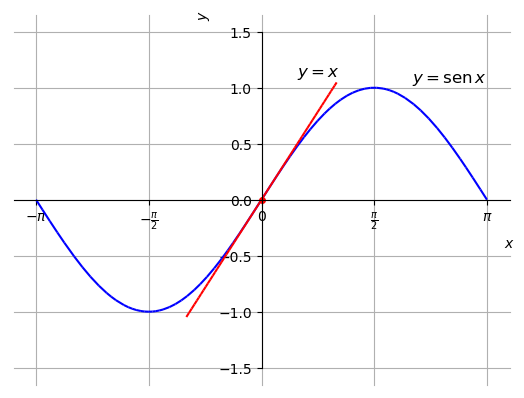
\includegraphics[width=0.7\textwidth]{./cap_deriv/dados/fig_deriv_exeresol_rt_sen0/fig_deriv_exeresol_rt_sen0}
    \caption{Esboços dos gráfico da função seno e de sua reta tangente no ponto $x=0$.}
    \label{fig:deriv_exeresol_rt_sen0}
  \end{figure}

  \ifispython
  Com o \sympy, podemos resolver este exercício com os seguintes comandos:
  \begin{lstlisting}
    from sympy import *
    x = Symbol('x')
    f = sin(x)
    x0 = 0

    # reta tangente
    rt = diff(f,x).subs(x,x0)*(x-x0)+f.subs(x,x0)
    print("Reta tangente: y = %s" % rt)

    # graficos
    plot(f,rt,(x,-pi,pi))
  \end{lstlisting}
  \fi  
\end{resol}

\begin{exeresol}
  Resolva a equação
  \begin{equation}
    \sec'(x) = 0,
  \end{equation}
  para $x\in \left(\frac{\pi}{2}, \frac{3\pi}{2}\right)$.
\end{exeresol}
\begin{resol}
  Temos
  \begin{align}
    0 &= \sec'(x) \\
      &= \sec(x)\tg(x) \\
      &= \frac{1}{\cos(x)}\frac{\sen(x)}{\cos(x)} \\
      &= \frac{\sen(x)}{\cos^2(x)}
  \end{align}
  donde segue que
  \begin{equation}
    \sen(x) = 0.
  \end{equation}
  Por fim, observamos que para $x\in \left(\frac{\pi}{2}, \frac{3\pi}{2}\right)$, a função seno se anula somente em $x=\pi$, a qual é a solução da equação.
\end{resol}


\subsection*{Exercícios}

\begin{flushright}
  [Vídeo] | [Áudio] | \href{https://phkonzen.github.io/notas/contato.html}{[Contatar]}
\end{flushright}

\begin{exer}
  Calcule a derivada em relação a $x$ de
  \begin{enumerate}[a)]
  \item $\displaystyle f(x)=\sen(x)-\cos^2(x)$
  \item $\displaystyle g(x)=\sen^2(x)\cos(x)$
  \item $\displaystyle h(x)=\frac{2\tg(x)}{\sec(x)}$
  \end{enumerate}
\end{exer}
\begin{resp}
  a)~$f'(x)=\sen(2x)+\cos(x)$; b)~$g'(x)=\sen(x)\cdot(2-3\sin^2(x)))$; c)~$h'(x)=2\cos(x)$
\end{resp}

\begin{exer}
  Encontre a equação da reta tangente ao gráfico da função $y = \cos x$ no ponto $x=0$. Então, faça os esboços desta função e da reta tangente, em uma mesma figura.  
\end{exer}
\begin{resp}
  $y = 1$. Dica: use um pacote de matemática simbólica para verificar os esboços dos gráficos.
\end{resp}

\begin{exer}
  Calcule a derivada em relação a $x$ de
  \begin{enumerate}[a)]
  \item $\displaystyle f(x)=\tg(x)-\cotg(x)$
  \item $\displaystyle g(x)=\sec(x)-\cossec(x)$
  \item $\displaystyle g(x)=\sec(x)-\cossec(x)$
  \end{enumerate}
\end{exer}
\begin{resp}
  a)~$f'(x)=\sec^2(x)+\cossec^2(x)$; b)~$g'(x)=\sec(x)\tg(x)+\cossec(x)\cotg(x)$; c)~$h'(x)=\frac{1}{2}\sec^2(x)$
\end{resp}


\section{Regra da cadeia}\label{cap_deriv_sec_cadeia}

\begin{flushright}
  [Vídeo] | [Áudio] | \href{https://phkonzen.github.io/notas/contato.html}{[Contatar]}
\end{flushright}

Regra da cadeia é nome dado a técnica de derivação de uma função composta. Sejam $f$ e $g$, com $g$ derivável em $x$ e $f$ derivável em $g(x)$, então $(f\circ g)$ é derivável em $x$, sendo
\begin{equation}
  \pmb{(f\circ g)'(x) = [f(g(x))]' = f'(g(x))\cdot g'(x)},
\end{equation}
chamada de regra da cadeia.

\begin{ex}
  A derivada em relação a $x$ de $h(x) = (x+1)^2$ pode ser calculada das seguintes formas:
  \begin{enumerate}
  \item[a)] pela regra da cadeia.

    A função $h$ é a composição da função $f(x)=x^2$ com a função $g(x)=x+1$, i.e. $h(x) = f(g(x))$. Temos $f'(x)=2x$ e $g'(x)=1$. Então, segue pela regra da cadeia
    \begin{align}
      h'(x) &= [f(g(x))]' \\
            &= f'(g(x))\cdot g'(x) \\
            &= 2(x+1)\cdot 1 \\
            &= 2x+2.
    \end{align}

  \item[b)] por cálculo direto.

    Observando que $h(x)=(x+1)^2=x^2+2x+1$, temos
    \begin{align}
      h'(x) &= (x^2+2x+1)' \\
            &= (x^2)' + (2x)' + (1)' \\
            &= 2x + 2.
    \end{align}
  \end{enumerate}

  \ifispython
  Com o \sympy, temos:
  \begin{lstlisting}
    from sympy import *
    x = Symbol('x')
    diff((x+1)**2,x)
    2*x + 2
  \end{lstlisting}
  \fi  
\end{ex}

Usualmente, a regra da cadeia também é apresentada da seguinte forma
\begin{equation}\label{eq:deriv_regra_da_cadeia}
  \pmb{\frac{\dd}{\dd x}f(u) = f'(u)\frac{\dd u}{\dd x}},
\end{equation}
onde $u$ é uma função derivável em $x$ e $f$ é derivável em $u(x)$.

\begin{ex}
  Vamos calcular a derivada em relação a $x$ de $g(x) = \sqrt{x^2+1}$. Temos que $g(x) = f(u(x))$, com $f(x) = \sqrt{x}$ e $u(x) = x^2+1$. Observando que
  \begin{equation}
    f'(x) = \frac{1}{2\sqrt{x}}\quad\text{e}\quad u'(x)=2x,
  \end{equation}
  segue pela regra da cadeia que
  \begin{align}
    g'(x) &= \frac{\dd}{\dd x}f(u) \\
          &= f'(u)\frac{\dd u}{\dd x} \\
          &= \frac{1}{2\sqrt{u}}\cdot 2x \\
          &= \frac{x}{\sqrt{x^2+1}}.
  \end{align}

  \ifispython
  No \sympy, temos:
\begin{lstlisting}
    from sympy import *
    x = Symbol('x')
    diff(sqrt(x**2+1),x)
    x/sqrt(x**2 + 1)
  \end{lstlisting}
  \fi  
\end{ex}

A regra da cadeia pode ser estendida para calcular a derivada de uma composição encadeada de três ou mais funções. Por exemplo,
\begin{equation}
  [f(g(h(x)))]' = f'(g(h(x)))\cdot[g(h(x))]' = f'(g(h(x)))\cdot g'(h(x))\cdot h'(x).
\end{equation}
Neste caso, a regra é válida para todo ponto tal que $h$ é derivável em $x$ com $g$ derivável em $h(x)$ e $f$ derivável em $f(g(h(x)))$.

\begin{ex}
  Vamos calcular a derivada em relação a $x$ de $f(x) = \sen(\cos(x^2))$. Pela regra da cadeia, temos
  \begin{align}
    [\sen(\cos(x^2))] &= \cos(\cos(x^2))\cdot[\cos(x^2)]' \\
                    &= \cos(\cos(x^2))\cdot [-\sen(x^2)\cdot (x^2)'] \\
                    &= -\cos(\cos(x^2))\cdot\sen(x^2)\cdot 2x.
  \end{align}

  \ifispython
  No \sympy, temos:
  \begin{lstlisting}
    from sympy import *
    x = Symbol('x')
    diff(sin(cos(x**2)))
    -2*x*sin(x**2)*cos(cos(x**2))
  \end{lstlisting}
  \fi  
\end{ex}

\subsection{Tabela de derivadas}

\begin{flushright}
  [Vídeo] | [Áudio] | \href{https://phkonzen.github.io/notas/contato.html}{[Contatar]}
\end{flushright}

\begin{align}
  & (ku)' = ku' && (u\pm v)' = u' \pm v'\\
  & (uv)' = u'v + uv' && \left(\frac{u}{v}\right)' = \frac{u'v - uv'}{v^2} \\
  & (k)' = 0 && \frac{\dd}{\dd x}u^n = nu^{n-1}\frac{\dd u}{\dd x}\\
  & \frac{\dd}{\dd x}a^u = a^u\ln a\frac{\dd u}{\dd x} && \frac{\dd}{\dd x}(e^u) = e^u\frac{\dd u}{\dd x} \\
  & \frac{\dd}{\dd x}\sen u = \cos(u)\frac{\dd u}{\dd x} && \frac{\dd}{\dd x}\cos u = - \sen(u)\frac{\dd u}{\dd x}\\
  & \frac{\dd}{\dd x}\tg u = \sec^2(u)\frac{\dd u}{\dd x} && \frac{\dd}{\dd x}\cotg u = -\cossec^2(u)\frac{\dd u}{\dd x} \\
  & \frac{\dd}{\dd x}\sec u = \sec(u)\tg(u)\frac{\dd u}{\dd x} && \frac{\dd}{\dd x}\cossec u = -\cossec(u)\cotg(u)\frac{\dd u}{\dd x}
\end{align}

\subsection*{Exercícios resolvidos}

\begin{flushright}
  [Vídeo] | [Áudio] | \href{https://phkonzen.github.io/notas/contato.html}{[Contatar]}
\end{flushright}

\begin{exeresol}
  Calcule a derivada em relação a $x$ de
  \begin{equation}
    f(x) = e^{\sqrt{x+1}}.
  \end{equation}
\end{exeresol}
\begin{resol}
  Da regra da cadeia aplicada à função exponencial, temos
  \begin{equation}
    \frac{\dd}{\dd x}e^u = e^u\frac{\dd u}{\dd x}.
  \end{equation}
  Então, com $u = \sqrt{x+1}$, segue
  \begin{align}
    f'(x) &= \frac{\dd}{\dd x}e^{\sqrt{x+1}} \\
          &= e^{\sqrt{x+1}}\frac{\dd}{\dd x}\left(\sqrt{x+1}\right).
  \end{align}
  Agora, aplicamos a regra da cadeia para a função raiz quadrada, i.e.
  \begin{equation}
    \frac{\dd}{\dd x}\sqrt{u} = \frac{1}{2\sqrt{u}}\frac{\dd u}{\dd x},
  \end{equation}
  com $u = x+1$. Segue, então
  \begin{align}
    \frac{\dd}{\dd x}\sqrt{x+1} &= \frac{1}{2}(x+1)^{\frac{1}{2}-1}\frac{\dd}{\dd x}(x+1) \\
                                &= \frac{1}{2\sqrt{x+1}}.
  \end{align}
  Portanto, concluímos que
  \begin{equation}
    f'(x) = \frac{1}{2\sqrt{x+1}}e^{\sqrt{x+1}}.
  \end{equation}

  \ifispython
  No \sympy, temos:
  \begin{lstlisting}
    from sympy import *
    x = Symbol('x')
    diff(exp(sqrt(x+1)),x)
    exp(sqrt(x + 1))/(2*sqrt(x + 1))
  \end{lstlisting}
  \fi  
\end{resol}

\begin{exeresol}
  Mostre que a \href{https://pt.wikipedia.org/wiki/Fun%C3%A7%C3%A3o_log%C3%ADstica}{função logística}
  \begin{equation}
    f(x) = \frac{1}{1+e^{-x}}
  \end{equation}
  satisfaz a equação diferencial
  \begin{equation}
    \frac{\dd}{\dd x}f(x) = f(x)(1-f(x)).
  \end{equation}
\end{exeresol}
\begin{resol}
  Vamos calcular a derivada em relação a $x$ da função logística, i.e.
  \begin{align}
    \frac{\dd}{\dd x}f(x) &= \frac{\dd}{\dd x}\left(\frac{1}{1+e^{-x}}\right) \\
          &= \frac{\dd}{\dd x}\left[\left(1+e^{-x}\right)^{-1}\right] \\
          &= -1\cdot\left(1+e^{-x}\right)^{-2}\cdot\underbrace{\left(1+e^{-x}\right)'}_{=-e^{-x}} \\
          &= \frac{e^{-x}}{\left(1+e^{-x}\right)^{2}}.
  \end{align}
  Por outro lado, temos
  \begin{align}
    f(x)(1-f(x)) &= \frac{1}{1+e^{-x}}\cdot\left(1 - \frac{1}{1+e^{-x}}\right) \\
                 &= \frac{1}{1+e^{-x}}\cdot\left(\frac{1+e^{-x}-1}{1+e^{-x}}\right) \\
                 &= \frac{e^{-x}}{\left(1+e^{-x}\right)^{2}}.
  \end{align}
  Ou seja, de fato temos
  \begin{equation}
    \frac{\dd}{\dd x}f(x) = f(x)(1-f(x)).
  \end{equation}  
\end{resol}

\begin{exeresol}
  Assuma que o custo de produção de uma unidade empresarial seja modelada pela função
  \begin{equation}
    c(x) = \sqrt{x-1} + e^{x-7},
  \end{equation}
  onde $c$ é o custo em função da produção $x$. Determine o custo marginal quando $x=3$.
\end{exeresol}
\begin{resol}
  O custo marginal é a função derivada do custo em relação à produção. Calculando, temos
  \begin{align}
    c'(x) &= \left(\sqrt{x-1} + e^{x-7}\right)\\
          &= \underbrace{\left(\sqrt{x-1}\right)'}_{(u^n)' = nu^{n-1}u'} + \underbrace{\left(e^{x-7}\right)'}_{(e^u)' = e^uu'}\\
          &= \frac{1}{2\sqrt{x-1}} + e^{x-7}.
  \end{align}
  Logo, o custo marginal quando $x=3$ é
  \begin{equation}
    c'(3) = \frac{1}{2\sqrt{3-1}} + e^{3-7} = \sqrt{2} + e^{-4}.
  \end{equation}
\end{resol}

\subsection*{Exercícios}

\begin{flushright}
  [Vídeo] | [Áudio] | \href{https://phkonzen.github.io/notas/contato.html}{[Contatar]}
\end{flushright}

\begin{ex}
  Calcule a derivada em relação a $x$ das seguintes funções
  \begin{enumerate}[a)]
  \item $\displaystyle f(x) = (2x-3)^{9}$
  \item $\displaystyle g(x) = \frac{1}{(2x-3)^{51}}$
  \end{enumerate}
\end{ex}
\begin{resp}
  a)~$\displaystyle f'(x) = 18(2x-3)^8$; b)~$\displaystyle g'(x) = -\frac{102}{(2x-3)^{52}}$;
\end{resp}

\begin{ex}
  Calcule a derivada em relação a $x$ das seguintes funções
  \begin{enumerate}[a)]
  \item $\displaystyle f(x) = 2^{3x-1}$
  \item $\displaystyle g(x) = e^{-x^2}$
  \end{enumerate}
\end{ex}
\begin{resp}
  a)~$\displaystyle f'(x) = 3\cdot 2^{3x-1}\ln 2$; b)~$\displaystyle g'(x) = -2xe^{-x^2}$.
\end{resp}

\begin{ex}
  Calcule a derivada em relação a $x$ das seguintes funções
  \begin{enumerate}[a)]
  \item $\displaystyle f(x) = \sen(\pi x)$
  \item $\displaystyle g(x) = \cos(\sqrt{x})$
  \item $\displaystyle h(x) = \tg(2x)$
  \item $\displaystyle u(x) = \cotg(3 - x)$
  \item $\displaystyle v(x) = \sec\left(\frac{1}{x^2}\right)$
  \item $\displaystyle z(x) = \cossec\left(5x + x^2\right)$
  \end{enumerate}
\end{ex}
\begin{resp}
  a)~$\displaystyle f'(x) = \pi\cos(\pi x)$; b)~$\displaystyle g'(x) = -\frac{1}{2\sqrt{x}}\sen(\sqrt{x})$; c)~$\displaystyle h'(x) = 2\sec^2(2x)$; d)~$\displaystyle u'(x) = \cossec^2(3-x)$; e)~$\displaystyle v'(x) = -\frac{2}{x^2}\sec\left(\frac{1}{x^2}\right)\tg\left(\frac{1}{x^2}\right)$; f)~$\displaystyle z'(x) = -(5+2x)\cossec\left(5x + x^2\right)\cotg\left(5x + x^2\right)$
\end{resp}

\begin{exer}
  Encontre a equação da reta tangente ao gráfico da função
  \begin{equation}
    f(x) = e^{\sqrt{x+1}}
  \end{equation}
  no ponto $x=3$.
\end{exer}
\begin{resp}
  $y = \frac{e^2}{4}x + \frac{e^2}{4}$
\end{resp}

\section{Diferenciabilidade da função inversa}\label{cap_deriv_sec_funinv}

\begin{flushright}
  [Vídeo] | [Áudio] | \href{https://phkonzen.github.io/notas/contato.html}{[Contatar]}
\end{flushright}

Seja $f$ uma função diferenciável e injetora em um intervalo aberto $I$. Então, pode-se mostrar que sua inversa $f^{-1}$ é diferenciável em qualquer ponto da imagem da $f$ no qual $f'(f^{-1}(x))\neq 0$ e sua derivada é
\begin{equation}\label{eq:diff_funinv}
  \pmb{\frac{d}{dx}[f^{-1}(x)] = \frac{1}{f'(f^{-1}(x))}}.
\end{equation}

\begin{ex}
  Seja $f(x) = (2x-1)^2$ para $x>1/2$. Para calcular sua inversa, fazemos
  \begin{gather}
    y = (2x-1)^2 \\
    \sqrt{y} = 2x-1 \\
    x = \frac{\sqrt{y}+1}{2}
  \end{gather}
  Ou seja,
  \begin{equation}
    f^{-1}(x) = \frac{1}{2}(\sqrt{x}+1).
  \end{equation}
  Calculando a derivada de $f^{-1}$ diretamente, temos
  \begin{align}
    \frac{\dd}{\dd x}f^{-1}(x) &= \frac{1}{2}\left(\sqrt{x}+1\right)' \\
                               &= \frac{1}{2}\cdot\frac{1}{2\sqrt{x}} \\
                               &= \frac{1}{4\sqrt{x}}
  \end{align}
  Agora, usando \eqref{eq:diff_funinv} e observando que $f'(x) = 8x-4$, obtemos
  \begin{align}
    \frac{\dd}{\dd x}f^{-1}(x) &= \frac{1}{f'(f^{-1}(x))},\\
                               &= \frac{1}{8\cdot \frac{1}{2}\left(\sqrt{x}+1\right)-4}, \\
                               &= \frac{1}{4\sqrt{x}},
  \end{align}
  como esperado.
\end{ex}

\begin{obs}\normalfont{(Derivada da função logarítmica)}
  \begin{itemize}
  \item Tomando $f(x) = e^x$ temos $f^{-1}(x) = \ln x$ e, daí por \eqref{eq:diff_funinv}
    \begin{equation}
      \frac{\dd }{\dd x}\ln x = \frac{1}{e^{\ln x}} = \frac{1}{x}.
    \end{equation}
  \item Tomando $f(x) = a^x$, $a> 0$ e $a\neq 1$, temos $f^{-1}(x) = \log_a x$ e, por \eqref{eq:diff_funinv},
    \begin{equation}
      \frac{\dd}{\dd x}\log_a x = \frac{1}{a^{\log_a x}\ln a} = \frac{1}{x\ln a}.
    \end{equation}
  \end{itemize}
\end{obs}

\begin{ex}
  Vamos calcular a derivada em relação a $x$ da função
  \begin{equation}
    f(x) = \ln \frac{1}{x}.
  \end{equation}
  Aplicando a regra da cadeia na derivada da função logarítmica, temos
  \begin{equation}
    \frac{\dd}{\dd x}\ln u = \frac{1}{u}\frac{\dd u}{\dd x}.
  \end{equation}
  Portanto, temos
  \begin{align}
    f'(x) &= \left(\ln\frac{1}{x}\right)'\\
          &= \frac{1}{x^{-1}}\cdot (-x^{-2}) \\
          &= -\frac{1}{x}.
  \end{align}

  \ifispython
  No \sympy, temos:
  \begin{lstlisting}
    from sympy import *
    x = Symbol('x')
    diff(log(1/x),x)
    -1/x
  \end{lstlisting}
  \fi  
\end{ex}

\begin{obs}\normalfont{(Derivada de função potência)}
  Em seções anteriores, já vimos que
  \begin{equation}
    \frac{\dd}{\dd x}x^n = nx^{n-1},
  \end{equation}
  para qualquer $n$ inteiro\footnote{Mais precisamente, para $n\neq 0$ e $n\neq 1$.}. Agora, se $r\neq 0$ e $r\neq 1$ é um número real, temos
  \begin{gather}
    y = x^r \\
    \ln y = \ln x^r = r\ln x.
  \end{gather}
  Daí, derivando ambos os lados desta última equação e observando que $y = y(x)$, obtemos
  \begin{gather}
    \frac{\dd}{\dd x} \ln y = \frac{\dd}{\dd x} r\ln x \\
    \frac{1}{y}\frac{\dd y}{\dd x} = \frac{r}{x} \\
    \frac{\dd y}{\dd x} = \frac{r}{x}y \\
    \frac{\dd y}{\dd x} = rx^{r-1}.
  \end{gather}
  Ou seja, a regra da potência
  \begin{equation}
    \frac{\dd}{\dd x}x^r = rx^{r-1},
  \end{equation}
  vale para todo $r$ real, com $r\neq 0$ e $r\neq 1$.
\end{obs}

\begin{ex}
  Vejamos os seguintes casos:
  \begin{enumerate}[a)]
  \item
    \begin{align}
      \frac{\dd}{\dd x}\sqrt{x} &= \left(x^{\frac{1}{2}}\right)' \\
                                &= \frac{1}{2}x^{\frac{1}{2}-1} \\
                                &= \frac{1}{2\sqrt{x}}.
    \end{align}
  \item
    \begin{align}
      \left(x^{\sqrt{2}}\right)' = \sqrt{2}x^{\sqrt{2}-1}.
    \end{align}
  \end{enumerate}
\end{ex}

\begin{ex}
  A regra da cadeia aplicada a derivada da função potência é
  \begin{equation}
    \frac{\dd}{\dd x}u^r = ru^{r-1}\frac{\dd u}{\dd x}.
  \end{equation}
  
  Por exemplo, temos
  \begin{align}
    \frac{\dd}{\dd x}\sqrt[3]{(x^2-1)} &= \frac{\dd}{\dd x}(x^2-1)^{\frac{1}{3}} \\
                                       &= \frac{2}{3}x\cdot (x^2-1)^{\frac{1}{3}-1} \\
                                       &= \frac{2}{3}x\cdot (x^2-1)^{-\frac{2}{3}} \\
                                       &= \frac{2x}{3\sqrt[3]{(x^2-1)^2}}.
  \end{align}
\end{ex}

\subsection{Derivadas de funções trigonométricas inversas}

\begin{flushright}
  [Vídeo] | [Áudio] | \href{https://phkonzen.github.io/notas/contato.html}{[Contatar]}
\end{flushright}

Seja $f(x) = \sen x$ restrita a $-\pi/2 \leq x \leq \pi/2$. Sua inversa é a função arco seno, denotada por
\begin{equation}
  y = \arc\sen x.
\end{equation}

\begin{figure}[H]
  \centering
  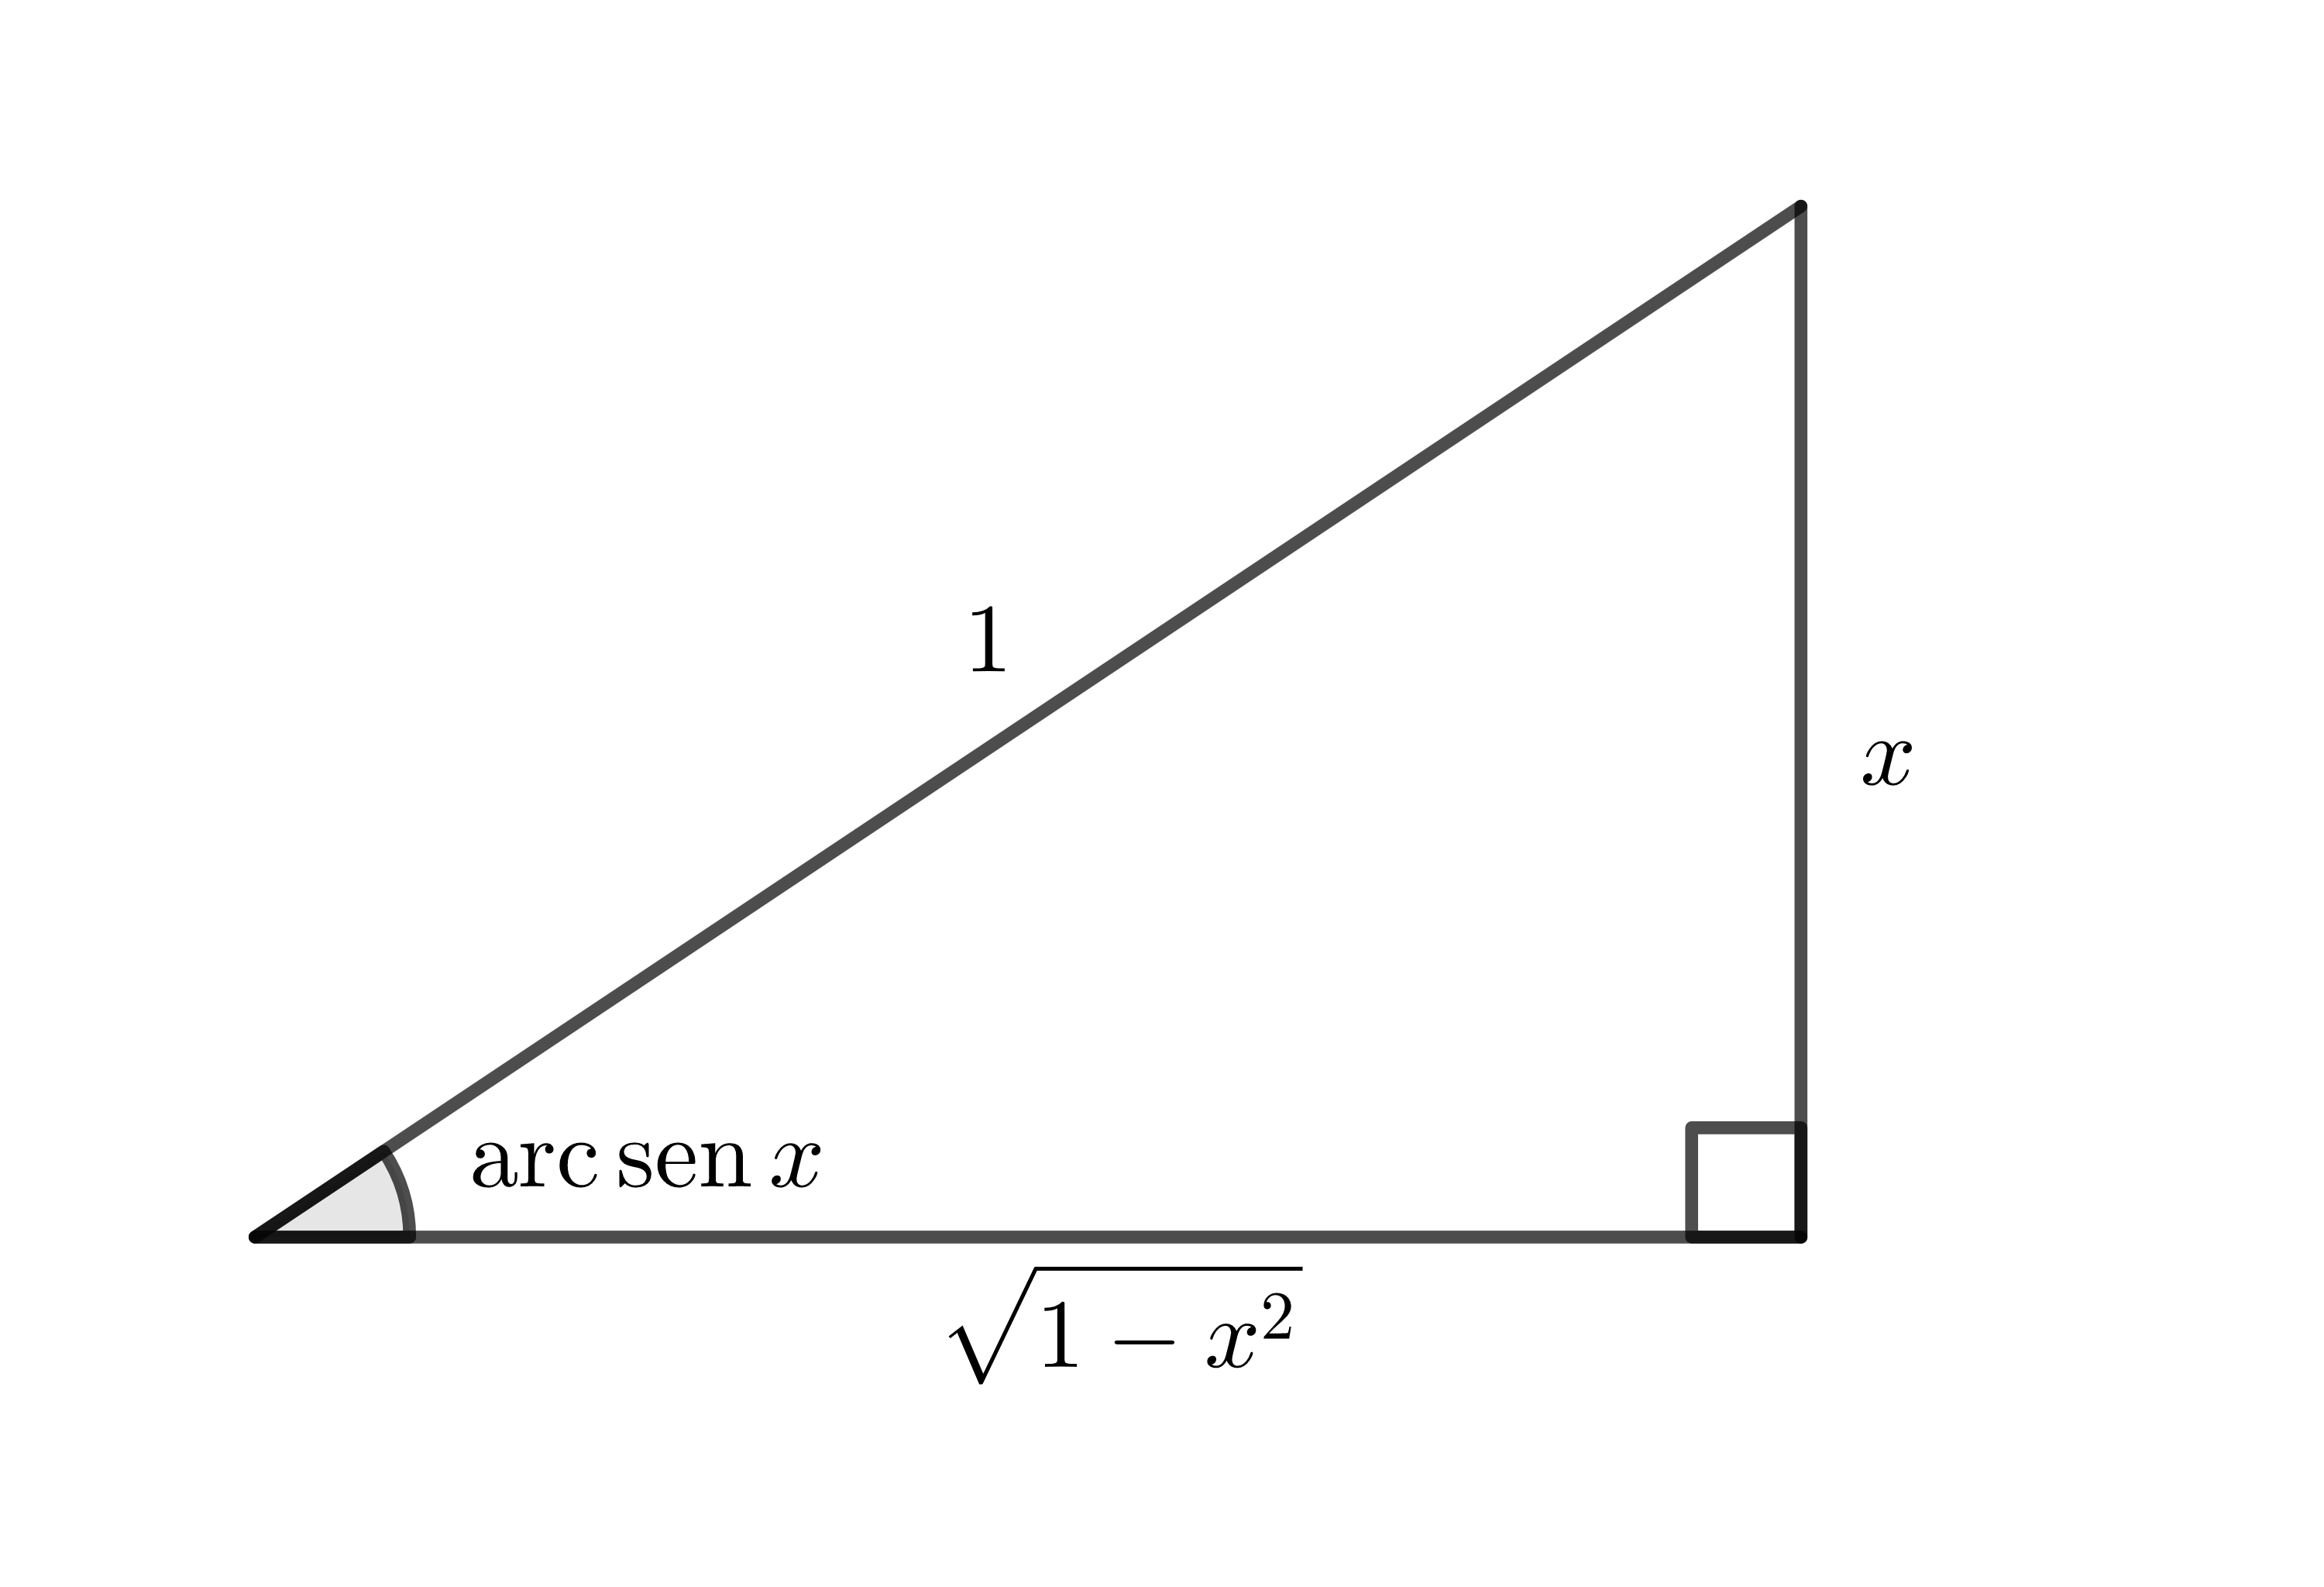
\includegraphics[width=0.5\textwidth]{./cap_deriv/dados/fig_diff_arc_sen/fig_diff_arc_sen}
  \caption{Arco seno de um ângulo no triângulo retângulo.}
  \label{fig:diff_arc_sen}
\end{figure}

Para calcular a derivada da função arco seno, vamos usar \eqref{eq:diff_funinv} com $f(x)=\sen x$ e $f'(x) = \arc\sen x$, donde
\begin{equation}
  (\arc\sen x)' = \frac{1}{\cos(\arc\sen x)}.
\end{equation}
Como $\cos(\arc\sen x) = \sqrt{1-x^2}$ (veja Figura \ref{fig:diff_arc_sen}), concluímos
\begin{equation}
  (\arc\sen x)' = \frac{1}{\sqrt{1-x^2}}.
\end{equation}


\begin{ex}
  A regra da cadeia aplicada à derivada da função arco seno é
  \begin{equation}
    \frac{\dd}{\dd x}\arc\sen u = \frac{1}{\sqrt{1-u^2}}\frac{\dd u}{\dd x}.
  \end{equation}

  Por exemplo, temos
  \begin{equation}
    \frac{\dd}{\dd x}\arc\sen x^2 = \frac{2x}{\sqrt{1-x^4}}.
  \end{equation}

  \ifispython
  No \sympy, temos:
  \begin{lstlisting}
    from sympy import *
    x = Symbol('x')
    diff(asin(x**2),x)
    2*x/sqrt(-x**4 + 1)
  \end{lstlisting}
  \fi    
\end{ex}

Com argumentos análogos aos usados no cálculo da derivada da função arco seno, podemos obter as seguintes derivadas:
\begin{align}
  & (\arc\cos x)' = -\frac{1}{\sqrt{1-x^2}} && \\
  &(\arc\tg x)' = \frac{1}{1+x^2} && (\arc\cotg x)' = -\frac{1}{1+x^2} \\
  & (\arc\sec x)' = \frac{1}{|x|\sqrt{x^2-1}} && (\arc\cosec x)' = -\frac{1}{|x|\sqrt{x^2-1}}
\end{align}

\begin{ex}
  A regra da cadeia aplicada a função arco tangente é
  \begin{equation}
    \frac{\dd}{\dd x}\arc\tg u = \frac{1}{1+u^2}\frac{\dd u}{\dd x}.
  \end{equation}

  Por exemplo, temos
  \begin{align}
    \frac{\dd}{\dd x}\arc\tg\sqrt{x} &= \frac{1}{1+(\sqrt{x})^2}\frac{\dd}{\dd x}\sqrt{x} \\
                                     &=  \frac{1}{2(1+x)\sqrt{x}}.
  \end{align}

  \ifispython
  No \sympy, temos:
  \begin{lstlisting}
    from sympy import *
    x = Symbol('x')
    diff(atan(sqrt(x)))
    1/(2*sqrt(x)*(x + 1))
  \end{lstlisting}
  \fi    
\end{ex}

\subsection{Tabela de derivadas}\label{deriv_tabela_de_derivadas}

\begin{flushright}
  [Vídeo] | [Áudio] | \href{https://phkonzen.github.io/notas/contato.html}{[Contatar]}
\end{flushright}

\begin{small}
\begin{align}
  & (ku)' = ku' && (u\pm v)' = u' \pm v'\\
  & (uv)' = u'v + uv' && \left(\frac{u}{v}\right)' = \frac{u'v - uv'}{v^2} \\
  & (k)' = 0 && \frac{\dd}{\dd x}u^r = ru^{r-1}\frac{\dd u}{\dd x}\\
  & \frac{\dd}{\dd x}a^u = a^u\ln a\frac{\dd u}{\dd x} && \frac{\dd}{\dd x}e^u = e^u\frac{\dd u}{\dd x} \\
  & \frac{\dd}{\dd x}\log_a u = \frac{1}{u\ln a}\frac{\dd u}{\dd x} && \frac{\dd}{\dd x}\ln u = \frac{1}{u}\frac{\dd u}{\dd x} \\
  & \frac{\dd}{\dd x}\sen u = \cos(u)\frac{\dd u}{\dd x} && \frac{\dd}{\dd x}\cos u = - \sen(u)\frac{\dd u}{\dd x}\\
  & \frac{\dd}{\dd x}\tg u = \sec^2(u)\frac{\dd u}{\dd x} && \frac{\dd}{\dd x}\cotg u = -\cossec^2(u)\frac{\dd u}{\dd x} \\
  & \frac{\dd}{\dd x}\sec u = \sec(u)\tg(u)\frac{\dd u}{\dd x} && \frac{\dd}{\dd x}\cossec u = -\cossec(u)\cotg(u)\frac{\dd u}{\dd x} \\
  &\frac{\dd}{\dd x}\arc\sen u = \frac{1}{\sqrt{1-u^2}}\frac{\dd u}{\dd x} && \frac{\dd}{\dd x}\arc\cos u = -\frac{1}{\sqrt{1-u^2}}\frac{\dd u}{\dd x} \\
  &\frac{\dd}{\dd x}\arc\tg u = \frac{1}{1+u^2}\frac{\dd u}{\dd x} && \frac{\dd}{\dd x}\arc\cotg u = -\frac{1}{1+u^2}\frac{\dd u}{\dd x} \\
  &\frac{\dd}{\dd x}\arc\sec u = \frac{1}{|u|\sqrt{u^2-1}}\frac{\dd u}{\dd x} && \frac{\dd}{\dd x}\arc\cossec u = -\frac{1}{|u|\sqrt{u^2-1}}\frac{\dd u}{\dd x}
\end{align}
\end{small}

\subsection*{Exercícios resolvidos}

\begin{flushright}
  [Vídeo] | [Áudio] | \href{https://phkonzen.github.io/notas/contato.html}{[Contatar]}
\end{flushright}

\begin{exeresol}
  Calcule a equação da reta tangente ao gráfico da função $f(x) = \ln x$ no ponto $x=1$. Faça, então, um esboço dos gráficos da função e da reta tangente.
\end{exeresol}
\begin{resol}
  A equação da reta tangente ao gráfico da função $f(x) = \ln x$ no ponto $x_0=1$ é
  \begin{gather}
    y = f'(x_0)(x-x_0)+f(x_0) \\
    y = f'(1)(x-1)+f(1).
  \end{gather}
  Observando que
  \begin{equation}
    f'(x) = (\ln x)' = \frac{1}{x},
  \end{equation}
  temos que a equação da reta tangente é
  \begin{gather}
    y = \frac{1}{1}(x-1)+\ln 1 \\
    y = x-1.
  \end{gather}
  Na Figura \ref{fig:deriv_exeresol_rt_ln}, temos um esboço dos gráficos da função e da reta tangente.

  \begin{figure}[H]
    \centering
    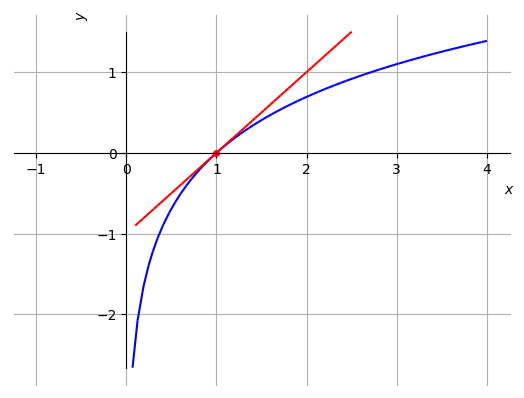
\includegraphics[width=0.7\textwidth]{./cap_deriv/dados/fig_deriv_exeresol_rt_ln/fig_deriv_exeresol_rt_ln}
    \caption{Esboço dos gráficos da função logarítmica natural e da reta tangente no ponto $x=1$.}
    \label{fig:deriv_exeresol_rt_ln}
  \end{figure}

  \ifispython
  No \sympy, temos:
  \begin{lstlisting}
    from sympy import *
    x = Symbol('x')
    rt = diff(log(x)).subs(x,1)*(x-1)+log(1)
    print("y = %s" % rt)
    y = x - 1
  \end{lstlisting}
  \fi    
\end{resol}

\begin{exeresol}
  Resolva a equação
  \begin{equation}
    \frac{\dd}{\dd x}\arc\tg x = 1.
  \end{equation}
\end{exeresol}
\begin{resol}
  Lembrando que
  \begin{equation}
    \frac{\dd}{\dd x}\arc\tg x = \frac{1}{1+x^2},
  \end{equation}
  temos
  \begin{gather}
    \frac{\dd}{\dd x}\arc\tg x = 1 \\
    \frac{1}{1+x^2}=1 \\
    1+x^2 = 1 \\
    x^2 = 0 \\
    x = 0.
  \end{gather}
\end{resol}

\begin{exeresol}
  Calcule
  \begin{equation}
    \frac{\dd}{\dd x}x^x.
  \end{equation}
\end{exeresol}
\begin{resol}
  Observamos que
  \begin{gather}
    y = x^x \\
    \ln y = \ln x^x \\
    \ln y = x\ln x.
  \end{gather}
  Agora, derivando em relação a $x$ ambos os lados desta equação, obtemos
  \begin{gather}
    \frac{\dd}{\dd x}\ln y = \frac{\dd}{\dd x}\left(x\ln x\right) \\
    \frac{1}{y}\frac{\dd y}{\dd x} = 1 + \ln x \\
    \frac{\dd y}{\dd x} = y(1 + \ln x) \\
    \frac{\dd x^x}{\dd x} = x^x(1 + \ln x).
  \end{gather}
\end{resol}

\subsection*{Exercícios}

\begin{flushright}
  [Vídeo] | [Áudio] | \href{https://phkonzen.github.io/notas/contato.html}{[Contatar]}
\end{flushright}

\begin{exer}
  Calcule a derivada em relação a $x$ das seguintes funções:
  \begin{enumerate}[a)]
  \item $f(x) = \log_2 x^2$
  \item $g(x) = \ln (xe^x)$
  \end{enumerate}
\end{exer}
\begin{resp}
  a)~$\displaystyle f'(x) = \frac{2}{x\ln 2}$; b)~$g'(x) = \frac{1+x}{x}$
\end{resp}

\begin{exer}
  Calcule a derivada em relação a $x$ das seguintes funções:
  \begin{enumerate}[a)]
  \item $f(x) = \sqrt[3]{x^2}$
  \item $g(x) = (1+2x)^e$
  \end{enumerate}
\end{exer}
\begin{resp}
  a)~$\displaystyle f'(x) = \frac{2}{3\sqrt[3]{x}}$; b)~$g'(x) = 2e(1+2x)^{e-1}$
\end{resp}

\begin{exer}
  Calcule
  \begin{equation}
    \frac{\dd}{\dd x} (1+x)^x.
  \end{equation}
\end{exer}
\begin{resp}
  $x(1+x)^{x-1} + (1+x)^x\ln(1+x)$
\end{resp}

\begin{exer}
  Encontre a equação da reta tangente ao gráfico de $f(x) = \arc\tg x$ no ponto $x=0$.
\end{exer}
\begin{resp}
  $y=x$
\end{resp}

\section{Derivação implícita}\label{cap_deriv_sec_derimp}

\begin{flushright}
  [Vídeo] | [Áudio] | \href{https://phkonzen.github.io/notas/contato.html}{[Contatar]}
\end{flushright}

Seja $y = y(x)$ definida implicitamente por
\begin{equation}
  g(y(x)) = 0.
\end{equation}
A derivada $\dd y/\dd x$ pode ser calculada via regra da cadeia
\begin{gather}
  \frac{\dd}{\dd x}g(y(x)) = \frac{\dd 0}{\dd x} \\
  g'(y(x))\frac{\dd y}{\dd x} = 0.
\end{gather}

\begin{ex}
  Considere a equação da circunferência unitária
  \begin{equation}
    x^2 + y^2 = 1.
  \end{equation}
  Para calcularmos $\dd y/\dd x$, fazemos
  \begin{gather}
    \frac{\dd}{\dd x}\left(x^2+y^2\right) = \frac{\dd 0}{\dd x} \\
    2x + \frac{\dd y^2}{\dd y}\frac{\dd y}{\dd x}\\
    2x + 2y\frac{\dd y}{\dd x} = 0\\
    \frac{\dd y}{\dd x} = -\frac{x}{y}.
  \end{gather}
\end{ex}

\subsection*{Exercícios resolvidos}

\begin{flushright}
  [Vídeo] | [Áudio] | \href{https://phkonzen.github.io/notas/contato.html}{[Contatar]}
\end{flushright}

\emconstrucao

\subsection*{Exercícios}

\begin{flushright}
  [Vídeo] | [Áudio] | \href{https://phkonzen.github.io/notas/contato.html}{[Contatar]}
\end{flushright}

\emconstrucao
